% \newcommand{\FigIdentifySender}{
% \begin{figure}[t]
%     \centering
%     \includegraphics[width=0.9\linewidth]{figures/linegraph.png}
%     \caption{\textbf{Messages needed to identify sender}\,---\,% 
%         We measured the number of epochs that were necessary for an attacker to
%         uniquely determine who was messaging a pre-selected victim, Bob, under
%         sealed sender assuming every message was ``immediately'' replied to with
%         a \textit{delivery receipt}. We found that the graph structure had no
%         influence on the effectiveness of the attack. We ran the attack 100
%         times for each user base size and found that with a user base of
%         1,000,000 on average Bob needed to receive 6.5 message from the same
%         user in order to deanonymize the conversation between the sender (Alice)
%         and Bob.
%         }
%     \label{fig:NumMessages}
% \end{figure}
% }

\newcommand{\SmallCountriesCorporate}{
    \begin{table}[t]
        \centering
        \small
        \scalebox{0.6}{
            \begin{tabular}{ccccccc}
                \toprule\textbf{Country} & \textbf{Resolver Pairs} & \textbf{IPv4 A} & \textbf{IPv4 AAAA} & \textbf{IPv6 A} & \textbf{IPv6 AAAA} & \textbf{Avg.}\\\midrule
                United States (US) & 757 & 1.62 & 1.16 & 0.54 & 0.96 & 1.07\\
                Germany (DE) & 717 & 0.98 & 0.91 & 0.75 & 0.80 & 0.86\\
                France (FR) & 470 & 0.60 & 0.45 & 0.40 & 0.46 & 0.48\\
                Great Britan (GB) & 186 & 1.07 & 0.94 & 0.78 & 0.97 & 0.94\\
                South Korea (KR) & 177 & 2.49 & 1.37 & 1.38 & 1.57 & 1.70\\
                Canada (CA) & 165 & 0.84 & 0.39 & 0.26 & 0.33 & 0.45\\
                Russia (RU) & 117 & 4.67 & 4.36 & 4.01 & 4.00 & 4.26\\
                India (IN) & 101 & 1.19 & 1.76 & 0.81 & 0.99 & 1.19\\
                Japan (JP) & 79 & 1.71 & 1.82 & 0.90 & 1.57 & 1.50\\
                South Africa (ZA) & 74 & 2.09 & 1.62 & 1.10 & 1.31 & 1.53\\
                Netherlands (NL) & 71 & 1.08 & 0.94 & 0.84 & 0.85 & 0.92\\
                Chile (CL) & 53 & 2.10 & 0.73 & 1.12 & 0.77 & 1.18\\
                Lithuania (LT) & 51 & 0.95 & 0.80 & 0.51 & 0.78 & 0.76\\
                Iran (IR) & 48 & 25.50 & 24.66 & 22.34 & 21.69 & 23.55\\
                Thailand (TH) & 43 & 9.28 & 1.18 & 0.99 & 0.95 & 3.10\\
                Singapore (SG) & 41 & 1.56 & 0.85 & 0.65 & 0.78 & 0.96\\
                Viet Nam (VN) & 40 & 2.16 & 1.01 & 0.85 & 0.86 & 1.22\\
                Hong Kong (HK) & 37 & 6.20 & 5.44 & 4.55 & 5.38 & 5.39\\
                Austrailia (AU) & 35 & 2.53 & 1.16 & 1.77 & 1.14 & 1.65\\
                Brazil (BR) & 34 & 1.50 & 1.10 & 1.01 & 1.17 & 1.19\\
                Finland (FI) & 31 & 0.74 & 0.64 & 0.47 & 0.56 & 0.60\\
                Malaysia (MY) & 30 & 6.07 & 2.25 & 0.97 & 1.10 & 2.60\\
                Spain (ES) & 28 & 1.26 & 0.97 & 2.24 & 2.97 & 1.86\\
                Turkey (TR) & 25 & 1.72 & 1.29 & 1.20 & 2.17 & 1.60\\
                \bottomrule
            \end{tabular}} 
            \caption{
                We highlight the countries with at least 25 resolver pairs in
                corporate ASes to showcase their censorship rates across
                interface and resource type. We see this is where the
                predominant censorship in the United States is present. 
            }
            \label{tab:small-countries-corporate}
    \end{table}
}


\newcommand{\IranRecursionTable}{
\begin{table}[h!]
    \begin{center}
        \begin{tabular}{l|c|c|c} % <-- Alignments: 1st column left, 2nd middle and 3rd right, with vertical lines in between
                  & \textbf{V4} & \textbf{V6} & \textbf{6to4}         \\
            \hline
            RD    & 10.10.34.35 & d0::11      & 10.10.34.35           \\
            No RD & 10.10.34.35 & d0::11      & \textbf{no injection} \\
        \end{tabular}
    \end{center}
    \caption{The Iranian censor provides distinctive injections to queries sent
        over both v4 and v6, but fails to inject responses for queries to
        resolvers using 6to4 addresses when the query excludes the recursion
        desired flag.}
    \label{tab:iran-recursion-table}
\end{table}
}

\newcommand{\CountriesCorporate}{
    \begin{table*}[ht]
        \centering
        {\tiny\renewcommand{\arraystretch}{.8}
        \resizebox{!}{.35\paperheight}{%
            \begin{tabular}{cccccccc}
                \toprule\textbf{Country} & \textbf{Network Type} & \textbf{Resolver Pairs} & \textbf{IPv4 A} & \textbf{IPv4 AAAA} & \textbf{IPv6 A} & \textbf{IPv6 AAAA} & \textbf{Avg.}\\\midrule
                CN & Total & 194 & 29.27 & 32.32 & 28.41 & 32.08 & 30.52\\                                                                                                                                                         
                CN & Corporate & 15 & 26.96 & 28.05 & 23.44 & 26.16 & 26.15\\                                                                                                                                                      
                CN & Non Corporate & 179 & 29.46 & 32.68 & 28.82 & 32.58 & 30.89\\                                                                                                                                                 
                \midrule                                                                                                                                                                                                           
                IR & Total & 277 & 25.12 & 24.49 & 21.95 & 21.45 & 23.25\\                                                                                                                                                         
                IR & Corporate & 48 & 25.50 & 24.66 & 22.34 & 21.69 & 23.55\\                                                                                                                                                      
                IR & Non Corporate & 229 & 25.04 & 24.46 & 21.87 & 21.40 & 23.19\\                                                                                                                                                 
                \midrule                                                                                                                                                                                                           
                HK & Total & 67 & 7.00 & 5.57 & 4.91 & 5.24 & 5.68\\                                                                                                                                                               
                HK & Corporate & 37 & 6.20 & 5.44 & 4.55 & 5.38 & 5.39\\                                                                                                                                                           
                HK & Non Corporate & 30 & 8.00 & 5.74 & 5.35 & 5.08 & 6.04\\                                                                                                                                                       
                \midrule                                                                                                                                                                                                           
                RU & Total & 312 & 5.51 & 4.78 & 4.49 & 4.50 & 4.82\\                                                                                                                                                              
                RU & Corporate & 117 & 4.67 & 4.36 & 4.01 & 4.00 & 4.26\\                                                                                                                                                          
                RU & Non Corporate & 195 & 6.02 & 5.03 & 4.78 & 4.80 & 5.16\\                                                                                                                                                      
                \midrule                                                                                                                                                                                                           
                UA & Total & 35 & 6.49 & 3.05 & 2.64 & 2.87 & 3.76\\                                                                                                                                                               
                UA & Corporate & 11 & 4.39 & 1.25 & 1.02 & 1.87 & 2.13\\                                                                                                                                                           
                UA & Non Corporate & 24 & 7.46 & 3.87 & 3.38 & 3.33 & 4.51\\                                                                                                                                                       
                \midrule                                                                                                                                                                                                           
                ID & Total & 56 & 6.46 & 2.99 & 2.41 & 2.26 & 3.53\\                                                                                                                                                               
                ID & Corporate & 16 & 6.92 & 3.38 & 3.02 & 2.83 & 4.04\\                                                                                                                                                           
                ID & Non Corporate & 40 & 6.27 & 2.84 & 2.17 & 2.04 & 3.33\\                                                                                                                                                       
                \midrule                                                                                                                                                                                                           
                AR & Total & 47 & 5.20 & 3.51 & 2.22 & 1.28 & 3.05\\                                                                                                                                                               
                AR & Corporate & 13 & 4.47 & 1.64 & 1.31 & 1.20 & 2.15\\                                                                                                                                                           
                AR & Non Corporate & 34 & 5.47 & 4.22 & 2.56 & 1.31 & 3.39\\                                                                                                                                                       
                \midrule                                                                                                                                                                                                           
                TH & Total & 186 & 8.25 & 1.18 & 1.13 & 0.93 & 2.87\\                                                                                                                                                              
                TH & Corporate & 43 & 9.28 & 1.18 & 0.99 & 0.95 & 3.10\\                                                                                                                                                           
                TH & Non Corporate & 143 & 7.94 & 1.18 & 1.17 & 0.93 & 2.80\\                                                                                                                                                      
                \midrule                                                                                                                                                                                                           
                MY & Total & 50 & 4.92 & 2.03 & 1.27 & 1.35 & 2.39\\                                                                                                                                                               
                MY & Corporate & 30 & 6.07 & 2.25 & 0.97 & 1.10 & 2.60\\                                                                                                                                                           
                MY & Non Corporate & 20 & 3.18 & 1.68 & 1.72 & 1.72 & 2.07\\                                                                                                                                                       
                \midrule                                                                                                                                                                                                           
                MX & Total & 150 & 3.78 & 2.05 & 1.75 & 1.94 & 2.38\\                                                                                                                                                              
                MX & Corporate & 10 & 2.04 & 2.27 & 2.41 & 2.54 & 2.31\\                                                                                                                                                           
                MX & Non Corporate & 140 & 3.90 & 2.03 & 1.70 & 1.89 & 2.38\\                                                                                                                                                      
                \midrule                                                                                                                                                                                                           
                BD & Total & 29 & 6.42 & 1.28 & 0.89 & 0.81 & 2.35\\                                                                                                                                                               
                BD & Corporate & 0 & 0.00 & 0.00 & 0.00 & 0.00 & 0.00\\
                BD & Non Corporate & 29 & 6.42 & 1.28 & 0.89 & 0.81 & 2.35\\
                \midrule
                CO & Total & 27 & 3.39 & 3.28 & 1.45 & 1.14 & 2.31\\ 
                CO & Corporate & 2 & 0.21 & 0.28 & 0.21 & 0.84 & 0.39\\
                CO & Non Corporate & 25 & 3.64 & 3.52 & 1.55 & 1.16 & 2.47\\
                \midrule
                IT & Total & 38 & 2.36 & 2.10 & 2.25 & 2.52 & 2.31\\ 
                IT & Corporate & 23 & 2.55 & 2.20 & 1.57 & 1.78 & 2.02\\
                IT & Non Corporate & 15 & 2.05 & 1.96 & 3.29 & 3.67 & 2.74\\
                \midrule
                BR & Total & 160 & 2.67 & 1.67 & 1.99 & 2.08 & 2.10\\
                BR & Corporate & 34 & 1.50 & 1.10 & 1.01 & 1.17 & 1.19\\
                BR & Non Corporate & 126 & 2.99 & 1.82 & 2.25 & 2.33 & 2.35\\
                \midrule
                BG & Total & 30 & 3.24 & 2.91 & 1.15 & 1.06 & 2.09\\
                BG & Corporate & 11 & 3.78 & 1.92 & 1.49 & 1.29 & 2.12\\
                BG & Non Corporate & 19 & 2.92 & 3.49 & 0.95 & 0.94 & 2.07\\
                \midrule
                PL & Total & 48 & 2.00 & 1.13 & 2.90 & 0.96 & 1.75\\
                PL & Corporate & 16 & 2.60 & 1.58 & 4.82 & 1.42 & 2.61\\
                PL & Non Corporate & 32 & 1.71 & 0.91 & 1.93 & 0.74 & 1.32\\
                \midrule
                ZA & Total & 93 & 2.41 & 1.60 & 1.18 & 1.33 & 1.63\\
                ZA & Corporate & 74 & 2.09 & 1.62 & 1.10 & 1.31 & 1.53\\
                ZA & Non Corporate & 19 & 3.64 & 1.53 & 1.48 & 1.42 & 2.02\\
                \midrule
                KR & Total & 632 & 2.33 & 1.06 & 1.24 & 1.22 & 1.46\\
                KR & Corporate & 177 & 2.49 & 1.37 & 1.38 & 1.57 & 1.70\\
                KR & Non Corporate & 455 & 2.26 & 0.94 & 1.19 & 1.09 & 1.37\\
                \midrule
                CL & Total & 65 & 2.67 & 0.70 & 1.10 & 0.79 & 1.32\\
                CL & Corporate & 53 & 2.10 & 0.73 & 1.12 & 0.77 & 1.18\\
                CL & Non Corporate & 12 & 5.17 & 0.58 & 1.00 & 0.91 & 1.92\\
                \midrule
                RO & Total & 44 & 2.30 & 1.03 & 0.83 & 0.93 & 1.27\\
                RO & Corporate & 6 & 2.17 & 0.58 & 0.47 & 0.63 & 0.96\\
                RO & Non Corporate & 38 & 2.32 & 1.10 & 0.89 & 0.97 & 1.32\\
                \midrule
                ES & Total & 49 & 0.91 & 0.75 & 1.40 & 1.94 & 1.25\\
                ES & Corporate & 28 & 1.26 & 0.97 & 2.24 & 2.97 & 1.86\\
                ES & Non Corporate & 21 & 0.46 & 0.47 & 0.29 & 0.58 & 0.45\\
                \midrule
                IN & Total & 226 & 1.27 & 1.52 & 1.04 & 1.16 & 1.25\\
                IN & Corporate & 101 & 1.19 & 1.76 & 0.81 & 0.99 & 1.19\\
                IN & Non Corporate & 125 & 1.34 & 1.32 & 1.23 & 1.30 & 1.30\\
                \midrule
                BE & Total & 31 & 1.56 & 1.26 & 0.95 & 0.95 & 1.18\\
                BE & Corporate & 4 & 1.33 & 1.30 & 1.16 & 1.26 & 1.26\\
                BE & Non Corporate & 27 & 1.59 & 1.25 & 0.92 & 0.91 & 1.17\\
                \midrule
                TR & Total & 114 & 1.29 & 0.96 & 1.27 & 1.02 & 1.14\\
                TR & Corporate & 25 & 1.72 & 1.29 & 1.20 & 2.17 & 1.60\\
                TR & Non Corporate & 89 & 1.17 & 0.86 & 1.29 & 0.70 & 1.01\\
                \midrule
                VN & Total & 252 & 1.53 & 0.89 & 1.42 & 0.67 & 1.13\\
                VN & Corporate & 40 & 2.16 & 1.01 & 0.85 & 0.86 & 1.22\\
                VN & Non Corporate & 212 & 1.42 & 0.86 & 1.52 & 0.64 & 1.11\\
                \bottomrule
            \end{tabular}}}
    \end{table*}
}

\newcommand{\IRTopDomainTable}{
    \begin{table}[t]
        \centering
        \begin{adjustbox}{width=\textwidth}
            \begin{tabular}{|c||ccc|}
                \hline\textbf{Domain} & \textbf{Requested Record Type} & \textbf{Number of Censoring v4 Resolvers} & \textbf{Number of Censoring v6 Resolvers}\\\hline
                secure.flickr.com & A & 276 & 209\\
                www.netflix.com & A & 275 & 206\\
                yumpu.com & A & 276 & 204\\
                www.urduvoa.com & A & 276 & 204\\
                www.snapchat.com & A & 274 & 206\\
                www.ning.com & A & 276 & 204\\
                www.lightsailvpn.com & A & 276 & 204\\
                signal.org & A & 275 & 205\\
                www.vonage.com & A & 276 & 203\\
                www.voanews.com & A & 276 & 203\\
                \hline
            \end{tabular}
        \end{adjustbox}
        \caption{\textbf{Iran table of most censored domains}\,---\,%
            We measured which domains were blocked in Iran, and whether they were
            blocked differently between resolvers at a v4 IP address, compared to
            those at a v6 IP address. As we can see here the most popularly blocked
            domains are blocked by resolvers on different IP address families but
            there is a difference. These domains were blocked by the most resolvers.
        }
        \label{tab:ir-top}
    \end{table}
}

\newcommand{\IRDifferenceDomainTable}{
    \begin{table}[ht]
        \centering
        \begin{adjustbox}{width=\textwidth}
            \begin{tabular}{|c||ccc|}
                \hline\textbf{Domain} & \textbf{Requested Record Type} & \textbf{Number of Censoring v4 Resolvers} & \textbf{Number of Censoring v6 Resolvers}\\\hline
                www.nbc.com & AAAA & 261 & 25\\
                download.cnet.com & AAAA & 259 & 23\\
                www.indiatimes.com & AAAA & 262 & 28\\
                spankbang.com & AAAA & 261 & 27\\
                psiphon.ca & AAAA & 261 & 27\\
                free.fr & AAAA & 261 & 27\\
                www.voanews.com & AAAA & 261 & 28\\
                www.netflix.com & AAAA & 262 & 29\\
                www.jesussaves.cc & AAAA & 261 & 28\\
                tmz.com & AAAA & 264 & 31\\
                \hline
            \end{tabular}
        \end{adjustbox}
        \caption{\textbf{Iran table of most difference in Address Family Censorship}\,---\,%
            We measured which domains were blocked in Iran, and whether they were
            blocked differently between resolvers at a v4 IP address, compared to
            those at a v6 IP address. As we can see here the most popularly blocked
            domains are blocked by resolvers on different IP address families but
            there is a difference. These domains had the largest difference in
            censoring behavior between resolver address family. 
        }
        \label{tab:ir-diff}
    \end{table}
}

\newcommand{\RUTopDomainTable}{
    \begin{table}[ht]
        \centering
        \begin{adjustbox}{width=\textwidth}
            \begin{tabular}{|c||ccc|}
                \hline\textbf{Domain} & \textbf{Requested Record Type} & \textbf{Number of Censoring v4 Resolvers} & \textbf{Number of Censoring v6 Resolvers}\\\hline
                eenadu.net & AAAA & 148 & 89\\
                www.spotify.com & AAAA & 93 & 98\\
                www.ned.org & A & 60 & 29\\
                www.europacasino.com & A & 47 & 37\\
                www.casinotropez.com & A & 45 & 37\\
                global.blackberry.com & A & 44 & 34\\
                www.sex.com & A & 40 & 37\\
                www.khilafah.com & A & 40 & 37\\
                ultrasurf.us & A & 41 & 36\\
                thepiratebay.org & A & 39 & 38\\
                \hline
            \end{tabular}
        \end{adjustbox}
        \caption{\textbf{Russia's top censored domains}\,---\,%
        }
        \label{tab:ru-top}
    \end{table}
}

\newcommand{\RUDifferenceDomainTable}{
    \begin{table}[ht]
        \centering
        \begin{adjustbox}{width=\textwidth}
            \begin{tabular}{|c||ccc|}
                \hline\textbf{Domain} & \textbf{Requested Record Type} & \textbf{Number of Censoring v4 Resolvers} & \textbf{Number of Censoring v6 Resolvers}\\\hline
                eenadu.net & AAAA & 148 & 89\\
                doh.dns.sb & A & 36 & 4\\
                www.ned.org & A & 60 & 29\\
                www.volcanomail.com & A & 30 & 0\\
                www.msf.org & A & 24 & 0\\
                mail.yahoo.com & A & 24 & 1\\
                www.cnn.com & AAAA & 0 & 21\\
                www.netflix.com & A & 27 & 10\\
                www.theglobalfund.org & A & 20 & 5\\
                www.ecdc.europa.eu & A & 15 & 0\\
                \hline
            \end{tabular}
        \end{adjustbox}
        \caption{\textbf{Russia's biggest difference domains}\,---\,%
        }
        \label{tab:ru-diff}
    \end{table}
}

\newcommand{\HKTopDomainTable}{
    \begin{table}[ht]
        \centering
        \begin{adjustbox}{width=\textwidth}
            \begin{tabular}{|c||ccc|}
                \hline\textbf{Domain} & \textbf{Requested Record Type} & \textbf{Number of Censoring v4 Resolvers} & \textbf{Number of Censoring v6 Resolvers}\\\hline
                eenadu.net & AAAA & 26 & 15\\
                www.ned.org & A & 14 & 3\\
                www.gov.uk & A & 12 & 2\\
                www.netflix.com & A & 11 & 2\\
                www.bittorrent.com & A & 10 & 2\\
                google.com.co & AAAA & 5 & 6\\
                www.nro.gov & A & 6 & 4\\
                www.terredeshommes.nl & A & 7 & 2\\
                mail.yahoo.com & A & 8 & 1\\
                google.ro & AAAA & 6 & 3\\
                \hline
            \end{tabular}
        \end{adjustbox}
        \caption{\textbf{Hong Kong's most censored domains}\,---\,%
        }
        \label{tab:hk-top}
    \end{table}
}

\newcommand{\HKDifferenceDomainTable}{
    \begin{table}[ht]
        \centering
        \begin{adjustbox}{width=\textwidth}
            \begin{tabular}{|c||ccc|}
                \hline\textbf{Domain} & \textbf{Requested Record Type} & \textbf{Number of Censoring v4 Resolvers} & \textbf{Number of Censoring v6 Resolvers}\\\hline
                www.ned.org & A & 14 & 3\\
                eenadu.net & AAAA & 26 & 15\\
                www.gov.uk & A & 12 & 2\\
                www.netflix.com & A & 11 & 2\\
                www.bittorrent.com & A & 10 & 2\\
                mail.yahoo.com & A & 8 & 1\\
                www.utorrent.com & A & 7 & 1\\
                www.ftchinese.com & A & 6 & 0\\
                www.familyequality.org & A & 7 & 1\\
                it.wikipedia.org & A & 6 & 0\\
                \hline
            \end{tabular}
        \end{adjustbox}
        \caption{\textbf{Hong Kong's biggest difference domains}\,---\,%
        }
        \label{tab:hk-diff}
    \end{table}
}

\newcommand{\CNTopDomainTable}{
    \begin{table}[ht]
        \centering
        \begin{adjustbox}{width=\textwidth}
            \begin{tabular}{|c||ccc|}
                \hline\textbf{Domain} & \textbf{Requested Record Type} & \textbf{Number of Censoring v4 Resolvers} & \textbf{Number of Censoring v6 Resolvers}\\\hline
                google.com.co & AAAA & 188 & 189\\
                google.co.in & AAAA & 189 & 188\\
                youtube.com & AAAA & 188 & 188\\
                www.ned.org & A & 189 & 187\\
                www.google.com & AAAA & 188 & 188\\
                www.blogger.com & AAAA & 188 & 188\\
                ultrasurf.us & AAAA & 188 & 188\\
                sites.google.com & AAAA & 188 & 188\\
                plus.google.com & AAAA & 188 & 188\\
                groups.google.com & AAAA & 188 & 188\\
                \hline
            \end{tabular}
        \end{adjustbox}
        \caption{\textbf{China's most censored domains}\,---\,%
        }
        \label{tab:cn-top}
    \end{table}
}

\newcommand{\CNDifferenceDomainTable}{
    \begin{table}[ht]
        \centering
        \begin{adjustbox}{width=\textwidth}
            \begin{tabular}{|c||ccc|}
                \hline\textbf{Domain} & \textbf{Requested Record Type} & \textbf{Number of Censoring v4 Resolvers} & \textbf{Number of Censoring v6 Resolvers}\\\hline
                google.com & A & 168 & 122\\
                google.com & AAAA & 180 & 145\\
                www.glaad.org & A & 30 & 6\\
                eenadu.net & AAAA & 116 & 96\\
                www.lanacion.com.ar & A & 20 & 1\\
                premierbet.co.ao & A & 25 & 7\\
                www.familyequality.org & A & 17 & 2\\
                www.bittorrent.com & A & 18 & 4\\
                qalam.withgoogle.com & A & 2 & 16\\
                global.blackberry.com & A & 16 & 2\\
                \hline
            \end{tabular}
        \end{adjustbox}
        \caption{\textbf{China's biggest difference domains}\,---\,%
        }
        \label{tab:cn-diff}
    \end{table}
}


% colors for the table below
%\definecolor{red0}{rgb}{1,0.9,0.9}
%\definecolor{red1}{rgb}{1,0.8,0.8}
%\definecolor{red2}{rgb}{1,0.7,0.7}
%\definecolor{red3}{rgb}{1,0.6,0.6}
%\definecolor{red4}{rgb}{1,0.5,0.5}
%\definecolor{red5}{rgb}{1,0.4,0.4}
%\definecolor{green0}{rgb}{0.9,1,0.9}
%\definecolor{green1}{rgb}{0.8,1,0.8}
%\definecolor{green2}{rgb}{0.7,1,0.7}
\definecolor{red00}{rgb}{1,0.9,0.9}
\definecolor{red0}{rgb}{1,0.8,0.8}
\definecolor{red1}{rgb}{1,0.7,0.7}
\definecolor{red2}{rgb}{1,0.6,0.6}
\definecolor{red3}{rgb}{1,0.5,0.5}
\definecolor{red4}{rgb}{1,0.4,0.4}
\definecolor{red5}{rgb}{1,0.3,0.3}
%\definecolor{green0}{rgb}{0.9,1,0.9}
\definecolor{green0}{rgb}{0.8,1,0.8}
\definecolor{green1}{rgb}{0.7,1,0.7}
\definecolor{green2}{rgb}{0.6,1,0.6}
\definecolor{green3}{rgb}{0.5,1,0.5}
\definecolor{green4}{rgb}{0.4,1,0.4}
\definecolor{green5}{rgb}{0.3,1,0.3}




\newcommand{\TabBaseRate}{
    \begin{table}[ht]
        \centering
        \small
        \scalebox{\tabularscale} {
        \begin{tabular}{lccccc}
            \toprule
                %\textbf{Country} & \textbf{Resolver pairs} & \textbf{v4/A} & \textbf{v4/AAAA} & \textbf{v6/A} & \textbf{v6/AAAA} \\
                \textbf{} & \textbf{Resolver} & \textbf{IPv4} & \textbf{IPv4} & \textbf{IPv6} & \textbf{IPv6} \\
                \textbf{Country} & \textbf{pairs} & \textbf{A} & \textbf{AAAA} & \textbf{A} & \textbf{AAAA} \\
                \midrule

United States (US)    &   1228  & 1.4\% & 0.9\% & 0.5\% & 0.9\% \\  % avg 0.9 stdev 2.6
Germany (DE)          &   753  & 1.0\% & 0.9\% & 0.8\% & 0.8\% \\  % avg 0.9 stdev 3.3
South Korea (KR)      &   632  & \cellcolor{red0} 2.3\% & 1.1\% & 1.2\% & 1.2\% \\  % avg 1.5 stdev 2.9
France (FR)           &   560  & 0.6\% & 0.5\% & 0.4\% & 0.6\% \\  % avg 0.5 stdev 1.8
Russia (RU)           &   312  & 5.5\% & 4.8\% & 4.5\% & 4.5\% \\  % avg 4.8 stdev 3.6
Iran (IR)             &   277  & \cellcolor{red1} 25.1\% & \cellcolor{red0} 24.5\% & \cellcolor{green0} 22.0\% & \cellcolor{green1} 21.4\% \\  % avg 23.3 stdev 3.4
Vietnam (VN)          &   252  & 1.5\% & 0.9\% & 1.4\% & 0.7\% \\  % avg 1.1 stdev 1.9
Taiwan (TW)           &   248  & 1.2\% & 1.0\% & 0.9\% & 0.9\% \\  % avg 1.0 stdev 4.0
India (IN)            &   226  & 1.3\% & 1.5\% & 1.0\% & 1.2\% \\  % avg 1.2 stdev 1.4
Canada (CA)           &   199  & \cellcolor{red0} 0.7\% & 0.4\% & 0.2\% & 0.3\% \\  % avg 0.4 stdev 1.2
United Kingdom (GB)   &   196  & 1.1\% & 0.9\% & 0.8\% & 1.0\% \\  % avg 1.0 stdev 3.3
China (CN)            &   194  & 29.3\% & \cellcolor{red0} 32.3\% & \cellcolor{green0} 28.4\% & \cellcolor{red0} 32.1\% \\  % avg 30.5 stdev 5.9
Thailand (TH)         &   186  & \cellcolor{red5}  8.2\% & \cellcolor{green0} 1.2\% & \cellcolor{green0} 1.1\% & \cellcolor{green0} 0.9\% \\  % avg 2.9 stdev 4.3
Brazil (BR)           &   160  & 2.7\% & 1.7\% & 2.0\% & 2.1\% \\  % avg 2.1 stdev 4.7
Japan (JP)            &   152  & 1.1\% & 1.2\% & 0.6\% & 1.0\% \\  % avg 1.0 stdev 3.4
Mexico (MX)           &   150  & \cellcolor{red0} 3.8\% & 2.0\% & 1.7\% & 1.9\% \\  % avg 2.4 stdev 5.0
Turkey (TR)           &   114  & 1.3\% & 1.0\% & 1.3\% & 1.0\% \\  % avg 1.1 stdev 3.2
Netherlands (NL)      &    97  & 1.2\% & 0.8\% & 0.7\% & 0.7\% \\  % avg 0.8 stdev 2.3
South Africa (ZA)     &    93  & 2.4\% & 1.6\% & 1.2\% & 1.4\% \\  % avg 1.6 stdev 4.2
Australia (AU)        &    72  & 1.6\% & 0.7\% & 0.9\% & 0.7\% \\  % avg 1.0 stdev 2.9
Hong Kong (HK)        &    67  & \cellcolor{red0} 7.0\% & 5.6\% & 4.9\% & 5.2\% \\  % avg 5.7 stdev 4.9
Chile (CL)            &    65  & \cellcolor{red1} 2.7\% & \cellcolor{green0} 0.7\% & 1.1\% & \cellcolor{green0} 0.8\% \\  % avg 1.3 stdev 1.8
Switzerland (CH)      &    60  & 0.3\% & 0.3\% & 0.3\% & 0.3\% \\  % avg 0.3 stdev 0.5
Indonesia (ID)        &    56  & \cellcolor{red0} 6.5\% & 3.0\% & 2.4\% & 2.3\% \\  % avg 3.5 stdev 6.3
Lithuania (LT)        &    52  & 0.9\% & 0.8\% & 0.5\% & 0.8\% \\  % avg 0.8 stdev 1.6
Singapore (SG)        &    50  & \cellcolor{red0} 1.8\% & 0.9\% & \cellcolor{green0} 0.6\% & 0.8\% \\  % avg 1.0 stdev 1.5
Malaysia (MY)         &    50  & \cellcolor{red1} 4.9\% & 2.0\% & \cellcolor{green0} 1.3\% & \cellcolor{green0} 1.4\% \\  % avg 2.4 stdev 3.5



                \hline
                %\textbf{Shown countries}            & \textbf{ 6501} & \textbf{3.8\%} & \textbf{3.2\%} & \textbf{2.8\%} & \textbf{3.0\%} \\
                \textbf{Global}            & \textbf{ 7441} & \textbf{3.6\%} & \textbf{3.0\%} & \textbf{2.6\%} & \textbf{2.7\%} \\
                \bottomrule
        \end{tabular}
        }
        \caption{\textbf{DNS censorship base rate}\,---\,%
            We discovered over 7,000 IPv4/IPv6 DNS resolver pairs around the world, and
            use them to measure censorship in their respective countries.
            We query each resolver pair (v4/v6 interfaces) with a list of over 700 domains
            from censorship lists that support both IPv4 and IPv6 addresses. For these domains,
            we request both \texttt{A} and \texttt{AAAA} records. We report on the average percent of censored
            responses for resolver inteface (v4 or v6) combined with record type (\texttt{A} or \texttt{AAAA}). Items significantly above (below) a country's average are colored red (green). We observe a general trend that IPv4 resolvers see more blocking than IPv6 resolvers.
            %and to a lesser extent, that IPv4 \texttt{A} records and IPv6 \texttt{AAAA} records are blocked more than IPv4 \texttt{AAAA} or IPv6 \texttt{A} records
            }
        \label{tab:base-rate}
    \end{table}
}


\newcommand{\TabBaseRateMedian}{
    \begin{table}[ht]
        \centering
        \small
        \scalebox{\tabularscale} {
        \begin{tabular}{lccccc}
            \toprule
                %\textbf{Country} & \textbf{Resolver pairs} & \textbf{v4/A} & \textbf{v4/AAAA} & \textbf{v6/A} & \textbf{v6/AAAA} \\
                \textbf{} & \textbf{Resolver} & \textbf{v4} & \textbf{v4} & \textbf{v6} & \textbf{v6} \\
                \textbf{Country} & \textbf{pairs} & \textbf{A} & \textbf{AAAA} & \textbf{A} & \textbf{AAAA} \\
                \midrule


                United States (US)    &   1228  & \cellcolor{green0} 0.1\% & 0.3\% & \cellcolor{green0} 0.1\% & 0.3\% \\  % avg 0.9 stdev 2.6 med 0.1
Germany (DE)          &   753  & 0.4\% & 0.4\% & 0.3\% & 0.4\% \\  % avg 0.9 stdev 3.3 med 0.4
South Korea (KR)      &   632  & 1.0\% & \cellcolor{green0} 0.6\% & \cellcolor{green0} 0.6\% & \cellcolor{green0} 0.6\% \\  % avg 1.5 stdev 2.9 med 0.6
France (FR)           &   560  & 0.1\% & 0.3\% & 0.1\% & 0.3\% \\  % avg 0.5 stdev 1.8 med 0.1
Russia (RU)           &   312  & 4.9\% & 4.9\% & 4.8\% & 4.9\% \\  % avg 4.8 stdev 3.6 med 4.9
Iran (IR)             &   277  & \cellcolor{red1} 25.4\% & \cellcolor{red0} 24.8\% & \cellcolor{green0} 21.8\% & \cellcolor{green0} 21.7\% \\  % avg 23.3 stdev 3.4 med 24.4
Vietnam (VN)          &   252  & 0.8\% & \cellcolor{green0} 0.4\% & \cellcolor{green0} 0.6\% & \cellcolor{green0} 0.4\% \\  % avg 1.1 stdev 1.9 med 0.6
Taiwan (TW)           &   248  & 0.3\% & 0.4\% & 0.3\% & 0.4\% \\  % avg 1.0 stdev 4.0 med 0.3
India (IN)            &   226  & 1.0\% & 1.0\% & \cellcolor{green0} 0.7\% & \cellcolor{green0} 0.8\% \\  % avg 1.2 stdev 1.4 med 0.8
Canada (CA)           &   199  & 0.3\% & 0.3\% & 0.1\% & 0.1\% \\  % avg 0.4 stdev 1.2 med 0.1
United Kingdom (GB)   &   196  & 0.3\% & 0.3\% & 0.1\% & 0.3\% \\  % avg 1.0 stdev 3.3 med 0.3
China (CN)            &   194  & \cellcolor{green0} 28.6\% & \cellcolor{red0} 32.1\% & \cellcolor{green0} 28.2\% & 31.9\% \\  % avg 30.5 stdev 5.9 med 31.4
Thailand (TH)         &   186  & \cellcolor{red5}  8.7\% & \cellcolor{green1} 0.6\% & \cellcolor{green1} 0.4\% & \cellcolor{green1} 0.4\% \\  % avg 2.9 stdev 4.3 med 0.6
Brazil (BR)           &   160  & \cellcolor{green0} 0.7\% & \cellcolor{green0} 0.6\% & \cellcolor{green0} 0.4\% & \cellcolor{green0} 0.6\% \\  % avg 2.1 stdev 4.7 med 0.6
Japan (JP)            &   152  & 0.1\% & 0.3\% & 0.1\% & 0.1\% \\  % avg 1.0 stdev 3.4 med 0.1
Mexico (MX)           &   150  & \cellcolor{green0} 0.4\% & \cellcolor{green0} 0.3\% & \cellcolor{green0} 0.1\% & \cellcolor{green0} 0.3\% \\  % avg 2.4 stdev 5.0 med 0.3
Turkey (TR)           &   114  & 0.7\% & 0.4\% & 0.4\% & 0.4\% \\  % avg 1.1 stdev 3.2 med 0.4
Netherlands (NL)      &    97  & \cellcolor{green0} 0.1\% & 0.3\% & \cellcolor{green0} 0.1\% & 0.3\% \\  % avg 0.8 stdev 2.3 med 0.3
South Africa (ZA)     &    93  & \cellcolor{green0} 0.4\% & 0.7\% & \cellcolor{green0} 0.3\% & \cellcolor{green0} 0.6\% \\  % avg 1.6 stdev 4.2 med 0.6
Australia (AU)        &    72  & 0.3\% & \cellcolor{green0} 0.1\% & \cellcolor{green0} 0.1\% & \cellcolor{green0} 0.1\% \\  % avg 1.0 stdev 2.9 med 0.1
Hong Kong (HK)        &    67  & 5.2\% & 4.8\% & 4.8\% & 4.8\% \\  % avg 5.7 stdev 4.9 med 4.8
Chile (CL)            &    65  & 1.3\% & \cellcolor{green0} 0.7\% & \cellcolor{green0} 0.7\% & \cellcolor{green0} 0.6\% \\  % avg 1.3 stdev 1.8 med 0.7
Switzerland (CH)      &    60  & \cellcolor{green0} 0.1\% & 0.3\% & \cellcolor{green0} 0.1\% & 0.3\% \\  % avg 0.3 stdev 0.5 med 0.1
Indonesia (ID)        &    56  & 4.9\% & \cellcolor{green0} 1.0\% & \cellcolor{green0} 1.0\% & \cellcolor{green0} 0.8\% \\  % avg 3.5 stdev 6.3 med 1.1
Lithuania (LT)        &    52  & 0.4\% & 0.6\% & 0.4\% & 0.4\% \\  % avg 0.8 stdev 1.6 med 0.4
Singapore (SG)        &    50  & 0.7\% & 0.7\% & \cellcolor{green0} 0.4\% & \cellcolor{green0} 0.6\% \\  % avg 1.0 stdev 1.5 med 0.6
Malaysia (MY)         &    50  & \cellcolor{red2} 5.2\% & \cellcolor{green0} 0.7\% & \cellcolor{green1} 0.4\% & \cellcolor{green1} 0.6\% \\  % avg 2.4 stdev 3.5 med 0.6

                \bottomrule
        \end{tabular}
        }
        \caption{\textbf{Base rate; medians}}
    \end{table}
}
 





\newcommand{\SomeCountryTable}{
    \begin{table}[ht]
        \centering
        \begin{tabular}{c|cc}
            \toprule
            \textbf{Country} & \textbf{Resolver pairs} & \textbf{Censored domains} \\
            \hline
                United States (US) & 1228 & 0\\
                Germany (DE) & 753 & 0\\
                South Korea (KR) & 632 & 0\\
                France (FR) & 560 & 0\\
                Russia (RU) & 312 & 30\\     % used to be 33??
                Iran (IR) & 277 & 169\\     % previously 172
                Vietnam (VN) & 252 & 0\\
                Taiwan (TW) & 248 & 0\\
                India (IN) & 226 & 0\\
                Canada (CA) & 199 & 0\\
                United Kingdom (GB) & 196 & 0\\
                China (CN) & 194 & 200\\
                Thailand (TH) & 186 & 0\\
                Brazil (BR) & 160 & 0\\
                Japan (JP) & 152 & 0\\
                Mexico (MX) & 150 & 0\\
                Turkey (TR) & 114 & 0\\     % used to be 3?
                Netherlands (NL) & 97 & 0\\
                South Africa (ZA) & 93 & 0\\
                Australia (AU) & 72 & 0\\
                Hong Kong (HK) & 67 & 30\\  % used to be 33
                Chile (CL) & 65 & 0\\
                Switzerland (CH) & 60 & 0\\
                Indonesia (ID) & 56 & 0\\
                Lithuania (LT) & 52 & 0\\
                Singapore (SG) & 50 & 0\\
                Malaysia (MY) & 50 & 0\\

                % UA & 35 & 1 \\        % dfas.mil
                % EG & 14 & 15 \\
                % KE & 8 & 2 \\
                % MO & 6 & 31 \\
                % AE & 6 & 6 \\
                % BY & 5 & 1 \\
                % TN & 2 & 1 \\
                % OM & 2 & 1 \\
                % MK & 2 & 47 \\
                % LA & 2 & 1 \\
                % IL & 2 & 30 \\
            \toprule
        \end{tabular}
        \caption{\textbf{DNS resolvers}\,---\,%
            We discovered over 7,000 IPv4/IPv6 DNS resolver pairs around the world, and
            use them to measure censorship in their respective countries.
            We queried each resolver with a list of over 700 domains from censorship
            lists that support both IPv4 and IPv6. We identify a domain as \texttt{censored}
            in a given country if over half of the country's resolvers blocked it.
            }
        \label{tab:country-resolvers}
    \end{table}
}

\newcommand{\FigIndiaCluster}{
    \begin{figure}[t]
     \centering
     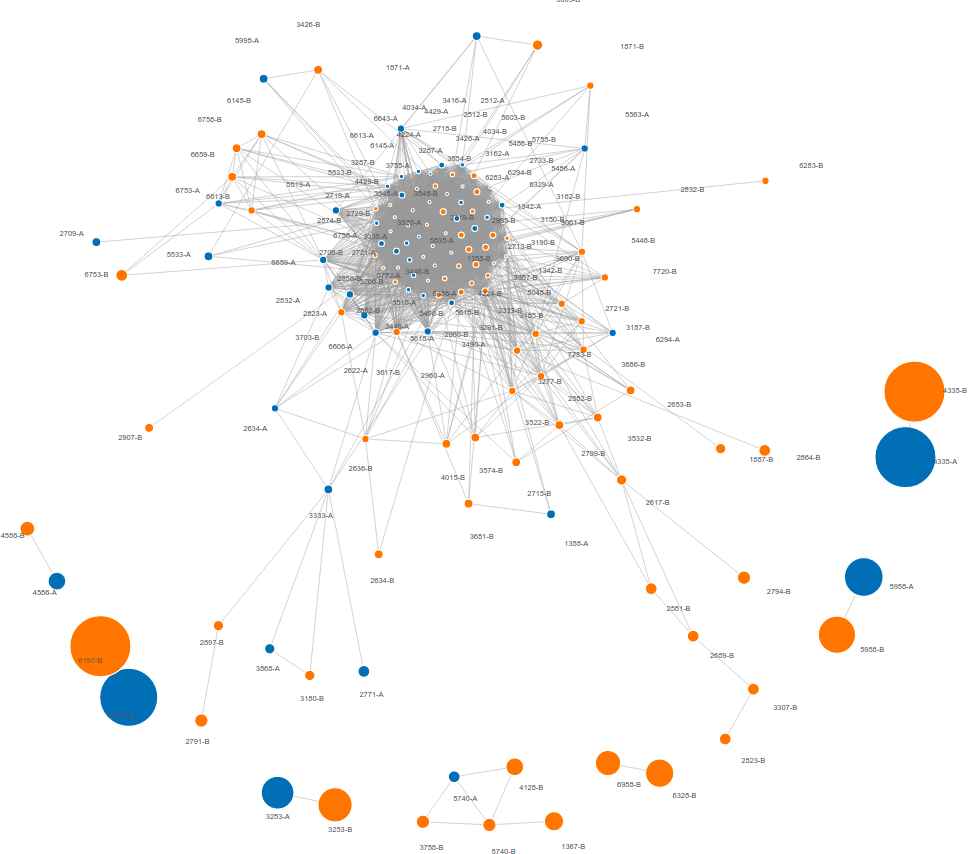
\includegraphics[width=0.9\linewidth]{figures/india.png}
     \caption{\textbf{India DNS censorship}\,---\,%
            We formed clusters of DNS resolvers using the levenshtein distance between
            the lists resolvers censor. Resolvers that block similar lists are connected,
            with node sizes proportional to the number of distinct domains blocked. We color
            IPv4 resolver interfaces blue, and IPv6 interfaces orange. This example illustrates
            the non-uniformity of India, with some ISPs censoring a large number of domains, and
            many others with small or non-existent block lists.}
    \label{fig:india}
    \end{figure}
}

\newcommand{\EveryCountryTable}{
    \begin{table}[ht]
        \centering
        {\tiny\renewcommand{\arraystretch}{.8}
        \resizebox{!}{.35\paperheight}{%
        \begin{tabular}{c|cc}
            \toprule
            \textbf{Country Code} & \textbf{Number of Resolver Pairs} & \textbf{Number of Censored Domains}\\
            \midrule
            US & 1228 & 0\\
            DE & 753 & 1\\
            KR & 632 & 2\\
            FR & 560 & 0\\
            RU & 312 & 33\\
            IR & 277 & 172\\
            VN & 252 & 2\\
            TW & 248 & 2\\
            IN & 226 & 2\\
            CA & 199 & 0\\
            GB & 196 & 0\\
            CN & 194 & 203\\
            TH & 186 & 2\\
            BR & 160 & 2\\
            JP & 152 & 0\\
            MX & 150 & 1\\
            TR & 114 & 3\\
            NL & 97 & 0\\
            ZA & 93 & 2\\
            AU & 72 & 0\\
            HK & 67 & 33\\
            CL & 65 & 2\\
            CH & 60 & 1\\
            ID & 56 & 2\\
            LT & 52 & 3\\
            SG & 50 & 3\\
            MY & 50 & 2\\
            ES & 49 & 0\\
            PL & 48 & 2\\
            AR & 47 & 2\\
            RO & 44 & 2\\
            CZ & 41 & 2\\
            IT & 38 & 1\\
            UA & 35 & 3\\
            SE & 34 & 0\\
            FI & 34 & 0\\
            BE & 31 & 1\\
            BG & 30 & 2\\
            BD & 29 & 3\\
            CO & 27 & 2\\
            SA & 24 & 2\\
            PK & 23 & 2\\
            HU & 22 & 1\\
            EC & 21 & 3\\
            GR & 20 & 0\\
            KZ & 19 & 0\\
            PH & 18 & 3\\
            NO & 16 & 0\\
            SK & 14 & 2\\
            EG & 14 & 17\\
            DK & 13 & 1\\
            PT & 11 & 0\\
            PE & 11 & 3\\
            NG & 9 & 2\\
            KE & 8 & 4\\
            AT & 8 & 1\\
            SI & 7 & 1\\
            RS & 7 & 0\\
            NZ & 7 & 1\\
            NP & 7 & 0\\
            MD & 7 & 0\\
            UY & 6 & 1\\
            MO & 6 & 32\\
            EE & 6 & 0\\
            CR & 6 & 3\\
            AE & 6 & 6\\
            VE & 5 & 2\\
            SD & 5 & 2\\
            PA & 5 & 0\\
            MN & 5 & 0\\
            LY & 5 & 1\\
            BY & 5 & 1\\
            AM & 5 & 1\\
            LV & 4 & 0\\
            LU & 4 & 0\\
            JO & 4 & 0\\
            IQ & 4 & 2\\
            GT & 4 & 0\\
            BZ & 4 & 1\\
            BO & 4 & 1\\
            BA & 4 & 1\\
            AL & 4 & 4\\
            LB & 3 & 1\\
            HR & 3 & 1\\
            HN & 3 & 1\\
            DO & 3 & 1\\
            AF & 3 & 0\\
            UG & 2 & 3\\
            TT & 2 & 0\\
            TN & 2 & 4\\
            TD & 2 & 2\\
            SV & 2 & 0\\
            OM & 2 & 2\\
            NI & 2 & 0\\
            MK & 2 & 49\\
            LA & 2 & 3\\
            IL & 2 & 31\\
            GU & 2 & 2\\
            GE & 2 & 2\\
            ET & 2 & 3\\
            CY & 2 & 3\\
            ZM & 1 & 5\\
            TZ & 1 & 4\\
            TG & 1 & 7\\
            SO & 1 & 1\\
            SC & 1 & 3\\
            PY & 1 & 8\\
            PF & 1 & 2\\
            MZ & 1 & 15\\
            MV & 1 & 11\\
            MM & 1 & 3\\
            MG & 1 & 7\\
            LK & 1 & 1\\
            LI & 1 & 1\\
            LC & 1 & 0\\
            KW & 1 & 1\\
            KG & 1 & 3\\
            HT & 1 & 0\\
            GI & 1 & 5\\
            GH & 1 & 2\\
            FJ & 1 & 2\\
            CM & 1 & 2\\
            AZ & 1 & 1\\
            AO & 1 & 4\\
            AI & 1 & 99\\
            PW & 0 & 3\\
            MA & 0 & 0\\
            KH & 0 & 4\\
            \bottomrule
        \end{tabular}}}
    \end{table}
}

\newcommand{\CompleteCountryTable}{
    \begin{table}[ht]
        \centering
        \begin{adjustbox}{width=\textwidth}
            \begin{tabular}{c|cc|cc|cc}
                \toprule
                \textbf{Country Code} & \textbf{Number of Resolver Pairs (January)} & \textbf{Number of Censored Domains (January)} & \textbf{Number of Resolver Pairs (December)} & \textbf{Number of Censored Domains (December)} & \textbf{Number of Resolver Pairs (November)} & \textbf{Number of Censored Domains (November)}\\
                \midrule
                US & 1228 & 0 & 1189 & 0 & 1201 & 0\\
                DE & 753 & 1 & 721 & 0 & 735 & 0\\
                KR & 632 & 2 & 504 & 2 & 595 & 2\\
                FR & 560 & 0 & 528 & 0 & 542 & 0\\
                RU & 312 & 33 & 296 & 32 & 316 & 33\\
                IR & 277 & 172 & 219 & 120 & 220 & 121\\
                VN & 252 & 2 & 179 & 2 & 214 & 2\\
                TW & 248 & 2 & 201 & 2 & 144 & 2\\
                IN & 226 & 2 & 181 & 2 & 185 & 2\\
                CA & 199 & 0 & 197 & 0 & 205 & 0\\
                GB & 196 & 0 & 196 & 0 & 190 & 0\\
                CN & 194 & 203 & 6 & 32 & 6 & 33\\
                TH & 186 & 2 & 144 & 3 & 202 & 2\\
                BR & 160 & 2 & 146 & 2 & 134 & 2\\
                JP & 152 & 0 & 138 & 0 & 142 & 0\\
                MX & 150 & 1 & 143 & 0 & 90 & 0\\
                TR & 114 & 3 & 90 & 2 & 102 & 2\\
                NL & 97 & 0 & 89 & 0 & 75 & 0\\
                ZA & 93 & 2 & 85 & 2 & 86 & 2\\
                AU & 72 & 0 & 65 & 0 & 71 & 0\\
                HK & 67 & 33 & 57 & 32 & 62 & 33\\
                CL & 65 & 2 & 46 & 2 & 63 & 2\\
                CH & 60 & 1 & 48 & 0 & 51 & 0\\
                ID & 56 & 2 & 31 & 2 & 53 & 2\\
                LT & 52 & 3 & 48 & 2 & 47 & 3\\
                SG & 50 & 3 & 29 & 2 & 39 & 3\\
                MY & 50 & 2 & 34 & 2 & 42 & 2\\
                ES & 49 & 0 & 46 & 0 & 54 & 0\\
                PL & 48 & 2 & 46 & 2 & 46 & 2\\
                AR & 47 & 2 & 47 & 2 & 55 & 2\\
                RO & 44 & 2 & 41 & 2 & 31 & 2\\
                CZ & 41 & 2 & 43 & 2 & 36 & 2\\
                IT & 38 & 1 & 29 & 0 & 31 & 0\\
                UA & 35 & 3 & 33 & 3 & 39 & 3\\
                SE & 34 & 0 & 34 & 0 & 35 & 0\\
                FI & 34 & 0 & 36 & 0 & 32 & 0\\
                BE & 31 & 1 & 32 & 0 & 26 & 0\\
                BG & 30 & 2 & 28 & 2 & 27 & 2\\
                BD & 29 & 3 & 7 & 3 & 21 & 2\\
                CO & 27 & 2 & 20 & 2 & 23 & 2\\
                SA & 24 & 2 & 15 & 2 & 11 & 2\\
                PK & 23 & 2 & 13 & 3 & 10 & 6\\
                HU & 22 & 1 & 16 & 0 & 15 & 1\\
                EC & 21 & 3 & 13 & 1 & 13 & 0\\
                GR & 20 & 0 & 13 & 0 & 15 & 0\\
                KZ & 19 & 0 & 14 & 1 & 21 & 0\\
                PH & 18 & 3 & 24 & 2 & 21 & 2\\
                NO & 16 & 0 & 16 & 0 & 13 & 0\\
                SK & 14 & 2 & 13 & 0 & 11 & 0\\
                EG & 14 & 17 & 13 & 16 & 2 & 27\\
                DK & 13 & 1 & 12 & 0 & 19 & 0\\
                PT & 11 & 0 & 15 & 0 & 11 & 0\\
                PE & 11 & 3 & 10 & 2 & 10 & 2\\
                NG & 9 & 2 & 7 & 3 & 6 & 2\\
                KE & 8 & 4 & 5 & 6 & 5 & 6\\
                AT & 8 & 1 & 11 & 0 & 8 & 1\\
                SI & 7 & 1 & 6 & 0 & 5 & 1\\
                RS & 7 & 0 & 6 & 0 & 4 & 0\\
                NZ & 7 & 1 & 5 & 0 & 6 & 0\\
                NP & 7 & 0 & 3 & 1 & 6 & 0\\
                MD & 7 & 0 & 5 & 0 & 1 & 1\\
                UY & 6 & 1 & 5 & 0 & 6 & 1\\
                MO & 6 & 32 & 7 & 31 & 4 & 31\\
                EE & 6 & 0 & 8 & 0 & 10 & 0\\
                CR & 6 & 3 & 6 & 2 & 4 & 0\\
                AE & 6 & 6 & 3 & 1 & 4 & 5\\
                VE & 5 & 2 & 4 & 2 & 5 & 2\\
                SD & 5 & 2 & 3 & 2 & 2 & 4\\
                PA & 5 & 0 & 3 & 0 & 4 & 0\\
                MN & 5 & 0 & 4 & 1 & 5 & 0\\
                LY & 5 & 1 & 4 & 3 & 5 & 2\\
                BY & 5 & 1 & 5 & 1 & 4 & 1\\
                AM & 5 & 1 & 2 & 5 & 2 & 1\\
                LV & 4 & 0 & 5 & 0 & 3 & 0\\
                LU & 4 & 0 & 3 & 0 & 3 & 0\\
                JO & 4 & 0 & 2 & 0 & 3 & 0\\
                IQ & 4 & 2 & 4 & 0 & 2 & 0\\
                GT & 4 & 0 & 5 & 0 & 6 & 0\\
                BZ & 4 & 1 & 3 & 1 & 2 & 1\\
                BO & 4 & 1 & 5 & 0 & 3 & 0\\
                BA & 4 & 1 & 3 & 1 & 3 & 0\\
                AL & 4 & 4 & 1 & 4 & 4 & 1\\
                LB & 3 & 1 & 2 & 0 & 2 & 0\\
                HR & 3 & 1 & 3 & 0 & 3 & 1\\
                HN & 3 & 1 & 3 & 0 & 1 & 0\\
                DO & 3 & 1 & 2 & 0 & 2 & 0\\
                AF & 3 & 0 & 2 & 3 & 3 & 4\\
                UG & 2 & 3 & 0 & -1 & 1 & 4\\
                TT & 2 & 0 & 2 & 1 & 2 & 0\\
                TN & 2 & 4 & 2 & 1 & 2 & 2\\
                TD & 2 & 2 & 2 & 2 & 2 & 2\\
                SV & 2 & 0 & 1 & 2 & 1 & 1\\
                OM & 2 & 2 & 1 & 2 & 1 & 0\\
                NI & 2 & 0 & 2 & 0 & 2 & 0\\
                MK & 2 & 49 & 1 & 2 & 2 & 50\\
                LA & 2 & 3 & 1 & 4 & 3 & 2\\
                IL & 2 & 31 & 4 & 0 & 4 & 0\\
                GU & 2 & 2 & 2 & 3 & 2 & 2\\
                GE & 2 & 2 & 2 & 3 & 3 & 1\\
                ET & 2 & 3 & 2 & 6 & 2 & 1\\
                CY & 2 & 3 & 2 & 2 & 3 & 3\\
                ZM & 1 & 5 & 0 & -1 & 0 & -1\\
                TZ & 1 & 4 & 1 & 5 & 1 & 7\\
                TG & 1 & 7 & 0 & -1 & 0 & 6\\
                SO & 1 & 1 & 1 & 3 & 1 & 2\\
                SC & 1 & 3 & 2 & 3 & 1 & 4\\
                PY & 1 & 8 & 2 & 7 & 2 & 6\\
                PF & 1 & 2 & 1 & 3 & 1 & 2\\
                MZ & 1 & 15 & 1 & 24 & 0 & -1\\
                MV & 1 & 11 & 0 & -1 & 0 & -1\\
                MM & 1 & 3 & 0 & -1 & 0 & -1\\
                MG & 1 & 7 & 1 & 5 & 2 & 6\\
                LK & 1 & 1 & 1 & 1 & 0 & -1\\
                LI & 1 & 1 & 1 & 1 & 1 & 2\\
                LC & 1 & 0 & 0 & -1 & 1 & 0\\
                KW & 1 & 1 & 1 & 1 & 1 & 1\\
                KG & 1 & 3 & 2 & 4 & 1 & 3\\
                HT & 1 & 0 & 0 & -1 & 0 & -1\\
                GI & 1 & 5 & 1 & 7 & 1 & 3\\
                GH & 1 & 2 & 1 & 2 & 2 & 2\\
                FJ & 1 & 2 & 0 & -1 & 0 & -1\\
                CM & 1 & 2 & 0 & -1 & 0 & -1\\
                AZ & 1 & 1 & 1 & 1 & 1 & 1\\
                AO & 1 & 4 & 1 & 2 & 1 & 3\\
                AI & 1 & 99 & 0 & -1 & 0 & -1\\
                PW & 0 & 3 & 1 & 1 & 1 & 1\\
                MA & 0 & 0 & 0 & 0 & 0 & -1\\
                KH & 0 & 4 & 3 & 2 & 0 & -1\\
                \bottomrule
            \end{tabular}
        \end{adjustbox}
    \end{table}
}



\newcommand{\TabBaseRateAllCountriesMedian}{
    \begin{table}[ht]
        \centering
        \small
        \scalebox{\tabularscale} {
        \begin{tabular}{lccccc}
            \toprule
                %\textbf{Country} & \textbf{Resolver pairs} & \textbf{v4/A} & \textbf{v4/AAAA} & \textbf{v6/A} & \textbf{v6/AAAA} \\
                \textbf{} & \textbf{Resolver} & \textbf{IPv4} & \textbf{IPv4} & \textbf{IPv6} & \textbf{IPv6} \\
                \textbf{Country} & \textbf{pairs} & \textbf{A} & \textbf{AAAA} & \textbf{A} & \textbf{AAAA} \\
                \midrule


Spain (ES)            &    49  & 0.4\% & 0.3\% & 0.1\% & 0.3\% \\  % avg 1.3 stdev 5.5 med 0.3
Poland (PL)           &    48  & 0.7\% & 0.6\% & 0.6\% & 0.4\% \\  % avg 1.7 stdev 5.7 med 0.6
Argentina (AR)        &    47  & 2.4\% & \cellcolor{green1} 0.8\% & \cellcolor{green1} 0.6\% & \cellcolor{green1} 0.4\% \\  % avg 3.0 stdev 4.4 med 0.7
Romania (RO)          &    44  & 0.7\% & \cellcolor{green0} 0.4\% & \cellcolor{green0} 0.4\% & \cellcolor{green0} 0.4\% \\  % avg 1.3 stdev 2.9 med 0.4
Czechia (CZ)          &    41  & 0.4\% & 0.6\% & 0.4\% & 0.6\% \\  % avg 0.9 stdev 2.0 med 0.4
Italy (IT)            &    38  & \cellcolor{green0} 0.7\% & \cellcolor{green0} 0.6\% & \cellcolor{green0} 0.4\% & \cellcolor{green0} 0.6\% \\  % avg 2.3 stdev 5.0 med 0.6
Sweden (SE)           &    34  & 0.1\% & 0.1\% & 0.1\% & 0.1\% \\  % avg 0.4 stdev 1.0 med 0.1
Finland (FI)          &    34  & \cellcolor{green0} 0.4\% & 0.6\% & \cellcolor{green0} 0.4\% & 0.6\% \\  % avg 0.6 stdev 0.4 med 0.6
Ukraine (UA)          &    34  & 3.1\% & \cellcolor{green0} 1.3\% & \cellcolor{green0} 0.8\% & \cellcolor{green0} 1.3\% \\  % avg 3.4 stdev 5.9 med 1.3
Belgium (BE)          &    31  & 0.6\% & \cellcolor{green0} 0.3\% & 0.4\% & \cellcolor{green0} 0.3\% \\  % avg 1.2 stdev 3.5 med 0.3
Bulgaria (BG)         &    30  & \cellcolor{green0} 0.4\% & \cellcolor{green0} 0.4\% & \cellcolor{green0} 0.4\% & \cellcolor{green0} 0.4\% \\  % avg 2.1 stdev 5.9 med 0.4
Bangladesh (BD)       &    29  & \cellcolor{red5}  8.3\% & \cellcolor{green0} 0.6\% & \cellcolor{green0} 0.6\% & \cellcolor{green0} 0.6\% \\  % avg 2.4 stdev 3.7 med 0.7
Colombia (CO)         &    27  & 1.8\% & \cellcolor{green0} 0.7\% & \cellcolor{green0} 0.7\% & \cellcolor{green0} 0.4\% \\  % avg 2.3 stdev 5.6 med 0.7
Saudi Arabia (SA)     &    24  & \cellcolor{green0} 0.7\% & \cellcolor{green0} 0.7\% & \cellcolor{green0} 0.4\% & \cellcolor{green0} 0.7\% \\  % avg 1.8 stdev 4.1 med 0.7
Pakistan (PK)         &    23  & \cellcolor{red1} 4.5\% & \cellcolor{green1} 1.7\% & \cellcolor{red0} 3.8\% & \cellcolor{green1} 1.4\% \\  % avg 3.0 stdev 2.2 med 2.1
Hungary (HU)          &    22  & \cellcolor{green1} 0.1\% & 0.3\% & \cellcolor{green1} 0.1\% & 0.3\% \\  % avg 0.3 stdev 0.3 med 0.3
Ecuador (EC)          &    21  & 1.1\% & 0.4\% & 0.4\% & 0.4\% \\  % avg 1.8 stdev 6.3 med 0.4
Greece (GR)           &    20  & \cellcolor{green0} 0.3\% & \cellcolor{green0} 0.3\% & \cellcolor{green0} 0.3\% & 0.4\% \\  % avg 0.7 stdev 1.4 med 0.3
Kazakhstan (KZ)       &    19  & \cellcolor{green0} 1.0\% & \cellcolor{green0} 0.8\% & \cellcolor{green0} 0.8\% & \cellcolor{green0} 1.0\% \\  % avg 2.4 stdev 4.3 med 0.8
Philippines (PH)      &    18  & 3.4\% & \cellcolor{green0} 1.7\% & \cellcolor{green1} 0.6\% & \cellcolor{green1} 0.6\% \\  % avg 2.8 stdev 4.0 med 1.3
Norway (NO)           &    16  & 0.3\% & \cellcolor{red0} 0.4\% & 0.3\% & \cellcolor{red0} 0.4\% \\  % avg 0.3 stdev 0.3 med 0.3
Egypt (EG)            &    14  & 3.4\% & 3.1\% & \cellcolor{green0} 2.4\% & \cellcolor{green0} 2.8\% \\  % avg 4.1 stdev 4.5 med 2.9
Slovakia (SK)         &    14  & 0.3\% & 0.3\% & 0.3\% & \cellcolor{red2} 0.4\% \\  % avg 0.2 stdev 0.2 med 0.3
Denmark (DK)          &    13  & \cellcolor{green0} 0.4\% & 0.6\% & \cellcolor{green0} 0.3\% & \cellcolor{green0} 0.3\% \\  % avg 1.2 stdev 3.0 med 0.4
Peru (PE)             &    11  & 1.0\% & \cellcolor{green0} 0.6\% & \cellcolor{green0} 0.6\% & \cellcolor{green0} 0.4\% \\  % avg 1.0 stdev 1.5 med 0.6
Portugal (PT)         &    11  & \cellcolor{green0} 0.1\% & \cellcolor{green0} 0.1\% & \cellcolor{green0} 0.0\% & \cellcolor{green0} 0.1\% \\  % avg 0.8 stdev 2.1 med 0.1
Nigeria (NG)          &     9  & 1.7\% & \cellcolor{green1} 0.6\% & 1.7\% & \cellcolor{green0} 1.3\% \\  % avg 2.0 stdev 2.5 med 1.7
Austria (AT)          &     8  & 0.1\% & \cellcolor{red2} 0.3\% & 0.1\% & 0.1\% \\  % avg 0.2 stdev 0.1 med 0.1
Kenya (KE)            &     8  & \cellcolor{red5}  9.9\% & \cellcolor{green0} 1.4\% & \cellcolor{green0} 1.1\% & \cellcolor{green0} 1.1\% \\  % avg 2.8 stdev 4.0 med 1.3
Moldova (MD)          &     7  & \cellcolor{green1} 0.1\% & \cellcolor{green1} 0.3\% & \cellcolor{green1} 0.3\% & \cellcolor{green1} 0.7\% \\  % avg 3.7 stdev 6.0 med 0.3
Serbia (RS)           &     7  & 0.1\% & \cellcolor{red1} 0.3\% & 0.1\% & \cellcolor{red1} 0.3\% \\  % avg 0.2 stdev 0.1 med 0.1
Slovenia (SI)         &     7  & \cellcolor{green0} 0.1\% & \cellcolor{green0} 0.3\% & \cellcolor{green0} 0.1\% & \cellcolor{green0} 0.1\% \\  % avg 1.0 stdev 2.4 med 0.1
New Zealand (NZ)      &     7  & \cellcolor{red5}  6.4\% & \cellcolor{green0} 0.1\% & 0.7\% & \cellcolor{green0} 0.1\% \\  % avg 1.3 stdev 2.5 med 0.1
Nepal (NP)            &     7  & 0.8\% & 0.8\% & \cellcolor{green1} 0.4\% & \cellcolor{green0} 0.7\% \\  % avg 1.0 stdev 0.8 med 0.7
Macao (MO)            &     6  & \cellcolor{green2} 4.3\% & 4.5\% & \cellcolor{green2} 4.3\% & 4.5\% \\  % avg 4.5 stdev 0.2 med 4.5
United Arab Emirates (AE)  &     6  & \cellcolor{red5}  1.7\% & \cellcolor{green1} 0.8\% & \cellcolor{green0} 1.0\% & \cellcolor{green0} 1.0\% \\  % avg 1.1 stdev 0.5 med 1.0
Estonia (EE)          &     6  & 0.6\% & 0.6\% & 0.4\% & 0.6\% \\  % avg 0.7 stdev 1.4 med 0.4
Costa Rica (CR)       &     6  & \cellcolor{red1} 7.3\% & \cellcolor{green0} 0.7\% & \cellcolor{green1} 0.6\% & \cellcolor{green1} 0.4\% \\  % avg 3.8 stdev 6.4 med 0.6
Uruguay (UY)          &     6  & \cellcolor{red1} 0.6\% & 0.4\% & \cellcolor{green0} 0.3\% & \cellcolor{green1} 0.1\% \\  % avg 0.4 stdev 0.3 med 0.3
Libya (LY)            &     5  & \cellcolor{green0} 0.4\% & 0.7\% & \cellcolor{green0} 0.4\% & \cellcolor{green0} 0.4\% \\  % avg 0.8 stdev 0.9 med 0.6
Mongolia (MN)         &     5  & \cellcolor{red0} 1.3\% & 0.8\% & 0.8\% & \cellcolor{green0} 0.7\% \\  % avg 1.0 stdev 0.9 med 0.8
Venezuela (VE)        &     5  & \cellcolor{red5}  8.0\% & \cellcolor{green0} 0.8\% & \cellcolor{green0} 0.7\% & \cellcolor{green0} 0.7\% \\  % avg 2.5 stdev 3.9 med 0.8
Belarus (BY)          &     5  & 0.8\% & \cellcolor{green1} 0.3\% & \cellcolor{green1} 0.3\% & 0.7\% \\  % avg 0.7 stdev 0.7 med 0.4
Armenia (AM)          &     5  & \cellcolor{green1} 0.4\% & \cellcolor{green2} 0.3\% & \cellcolor{green1} 0.4\% & 0.7\% \\  % avg 0.7 stdev 0.6 med 0.4
Panama (PA)           &     5  & 1.7\% & \cellcolor{green0} 0.8\% & \cellcolor{green0} 0.3\% & \cellcolor{green0} 0.3\% \\  % avg 2.1 stdev 4.1 med 0.7
Sudan (SD)            &     5  & 3.1\% & 3.8\% & \cellcolor{green1} 1.3\% & \cellcolor{green1} 1.4\% \\  % avg 3.4 stdev 3.0 med 2.8
Bosnia and Herzegovina (BA)  &     4  & \cellcolor{red1} 2.1\% & \cellcolor{green0} 0.4\% & \cellcolor{green0} 0.4\% & \cellcolor{green0} 0.4\% \\  % avg 1.1 stdev 1.5 med 0.4
Guatemala (GT)        &     4  & 0.4\% & \cellcolor{red0} 0.6\% & \cellcolor{green1} 0.3\% & \cellcolor{green1} 0.3\% \\  % avg 0.4 stdev 0.3 med 0.4
Luxembourg (LU)       &     4  & 0.1\% & 0.1\% & \cellcolor{green0} 0.0\% & 0.1\% \\  % avg 0.6 stdev 1.7 med 0.1
Iraq (IQ)             &     4  & \cellcolor{green0} 1.0\% & \cellcolor{green0} 0.8\% & \cellcolor{green0} 1.0\% & \cellcolor{green0} 1.1\% \\  % avg 2.6 stdev 3.7 med 0.8
Latvia (LV)           &     4  & \cellcolor{green2} 0.0\% & 0.1\% & 0.1\% & 0.1\% \\  % avg 0.1 stdev 0.1 med 0.1
Albania (AL)          &     4  & \cellcolor{green0} 0.4\% & 0.6\% & \cellcolor{green0} 0.4\% & \cellcolor{green0} 0.4\% \\  % avg 0.5 stdev 0.3 med 0.4
Jordan (JO)           &     4  & 0.3\% & 0.3\% & \cellcolor{green1} 0.1\% & \cellcolor{red2} 0.6\% \\  % avg 0.3 stdev 0.3 med 0.3
Belize (BZ)           &     4  & \cellcolor{red5}  8.7\% & \cellcolor{green0} 0.6\% & \cellcolor{green0} 0.6\% & \cellcolor{green0} 0.4\% \\  % avg 1.8 stdev 3.0 med 0.6
Bolivia (BO)          &     4  & 0.6\% & 0.6\% & \cellcolor{green0} 0.3\% & 0.4\% \\  % avg 0.6 stdev 0.7 med 0.4
Croatia (HR)          &     3  & \cellcolor{green1} 0.1\% & \cellcolor{red5}  0.3\% & \cellcolor{green1} 0.1\% & \cellcolor{green1} 0.1\% \\  % avg 0.2 stdev 0.1 med 0.1
Lebanon (LB)          &     3  & \cellcolor{red5}  0.7\% & 0.4\% & 0.4\% & 0.4\% \\  % avg 0.4 stdev 0.2 med 0.4
Afghanistan (AF)      &     3  & \cellcolor{red2} 2.7\% & \cellcolor{green0} 1.4\% & \cellcolor{green0} 1.4\% & 1.5\% \\  % avg 1.8 stdev 1.1 med 1.5
Honduras (HN)         &     3  & 1.3\% & \cellcolor{red1} 1.5\% & \cellcolor{green1} 0.4\% & \cellcolor{green1} 0.4\% \\  % avg 1.1 stdev 0.9 med 1.1
Dominican Republic (DO)  &     3  & \cellcolor{red5}  6.0\% & \cellcolor{green0} 0.6\% & \cellcolor{green1} 0.3\% & \cellcolor{green0} 0.4\% \\  % avg 1.6 stdev 2.3 med 0.6
North Macedonia (MK)  &     2  & \cellcolor{red5}  18.9\% & \cellcolor{red2} 12.6\% & \cellcolor{red0} 9.1\% & \cellcolor{red0} 9.5\% \\  % avg 6.4 stdev 6.8 med 9.1
Georgia (GE)          &     2  & \cellcolor{red2} 2.2\% & \cellcolor{red5}  2.4\% & \cellcolor{red5}  2.7\% & \cellcolor{red1} 1.8\% \\  % avg 1.2 stdev 1.1 med 1.8
Israel (IL)           &     2  & \cellcolor{red5}  5.2\% & \cellcolor{red5}  5.2\% & \cellcolor{red2} 5.0\% & \cellcolor{red5}  5.2\% \\  % avg 2.8 stdev 2.4 med 5.0
Lao People's Democratic Republic (LA)  &     2  & \cellcolor{red5}  9.7\% & \cellcolor{green0} 0.8\% & \cellcolor{green1} 0.4\% & \cellcolor{green1} 0.6\% \\  % avg 2.6 stdev 3.9 med 0.6
El Salvador (SV)      &     2  & \cellcolor{red5}  1.1\% & 0.4\% & \cellcolor{green2} 0.1\% & \cellcolor{green0} 0.3\% \\  % avg 0.4 stdev 0.3 med 0.3
Chad (TD)             &     2  & \cellcolor{red5}  5.5\% & \cellcolor{red0} 2.1\% & 1.3\% & \cellcolor{red0} 2.2\% \\  % avg 1.4 stdev 1.7 med 1.3
Nicaragua (NI)        &     2  & \cellcolor{red5}  7.1\% & \cellcolor{green0} 0.4\% & 0.7\% & \cellcolor{green0} 0.1\% \\  % avg 1.1 stdev 2.3 med 0.4
Uganda (UG)           &     2  & \cellcolor{green0} 0.8\% & \cellcolor{green0} 0.7\% & \cellcolor{green0} 1.0\% & \cellcolor{red5}  13.0\% \\  % avg 2.0 stdev 4.2 med 0.7
Guam (GU)             &     2  & \cellcolor{red5}  8.7\% & \cellcolor{green1} 0.4\% & \cellcolor{green1} 0.0\% & \cellcolor{green1} 0.4\% \\  % avg 2.2 stdev 3.4 med 0.4
Trinidad and Tobago (TT)  &     2  & \cellcolor{red5}  0.6\% & \cellcolor{red2} 0.3\% & 0.1\% & \cellcolor{green2} 0.0\% \\  % avg 0.1 stdev 0.2 med 0.1
Tunisia (TN)          &     2  & \cellcolor{red1} 0.6\% & \cellcolor{red1} 0.6\% & \cellcolor{red1} 0.6\% & \cellcolor{red5}  0.8\% \\  % avg 0.4 stdev 0.2 med 0.6
Ethiopia (ET)         &     2  & \cellcolor{green0} 0.3\% & \cellcolor{green0} 0.7\% & \cellcolor{red5}  51.1\% & \cellcolor{green0} 0.6\% \\  % avg 6.7 stdev 16.8 med 0.4
Oman (OM)             &     2  & \cellcolor{red5}  10.8\% & 1.3\% & \cellcolor{green0} 0.7\% & 1.0\% \\  % avg 1.8 stdev 3.4 med 0.7
Cyprus (CY)           &     2  & \cellcolor{red5}  9.5\% & 1.4\% & \cellcolor{green0} 0.6\% & \cellcolor{green0} 0.6\% \\  % avg 1.6 stdev 3.0 med 0.6
Liechtenstein (LI)    &     1  & \cellcolor{green5}  0.0\% & \cellcolor{green0} 0.1\% & \cellcolor{green0} 0.1\% & \cellcolor{red5}  0.6\% \\  % avg 0.2 stdev 0.2 med 0.1
Madagascar (MG)       &     1  & \cellcolor{red0} 1.1\% & \cellcolor{red5}  1.4\% & \cellcolor{green5}  0.4\% & \cellcolor{red0} 1.1\% \\  % avg 1.0 stdev 0.4 med 1.1
Myanmar (MM)          &     1  & \cellcolor{red5}  0.7\% & \cellcolor{red5}  0.7\% & \cellcolor{green5}  0.3\% & \cellcolor{green5}  0.3\% \\  % avg 0.5 stdev 0.2 med 0.7
Zambia (ZM)           &     1  & \cellcolor{red5}  2.8\% & \cellcolor{green1} 0.8\% & \cellcolor{green1} 0.8\% & \cellcolor{green1} 0.8\% \\  % avg 1.3 stdev 0.8 med 0.8
Kyrgyzstan (KG)       &     1  & \cellcolor{green5}  0.4\% & \cellcolor{red5}  2.7\% & \cellcolor{red2} 2.4\% & \cellcolor{green1} 1.0\% \\  % avg 1.6 stdev 0.9 med 2.4
Ghana (GH)            &     1  & \cellcolor{red5}  8.8\% & \cellcolor{green0} 0.8\% & \cellcolor{green1} 0.1\% & \cellcolor{green1} 0.4\% \\  % avg 2.6 stdev 3.6 med 0.8
Gibraltar (GI)        &     1  & \cellcolor{red5}  1.3\% & \cellcolor{red0} 1.0\% & \cellcolor{green1} 0.7\% & \cellcolor{green5}  0.6\% \\  % avg 0.9 stdev 0.3 med 1.0
Haiti (HT)            &     1  & \cellcolor{red5}  8.5\% & \cellcolor{green1} 0.3\% & \cellcolor{green1} 0.4\% & \cellcolor{green1} 0.0\% \\  % avg 2.3 stdev 3.6 med 0.4
Togo (TG)             &     1  & \cellcolor{red5}  3.9\% & \cellcolor{green0} 1.5\% & \cellcolor{green5}  0.8\% & 1.8\% \\  % avg 2.0 stdev 1.1 med 1.8
Somalia (SO)          &     1  & \cellcolor{red5}  6.0\% & \cellcolor{green1} 0.6\% & \cellcolor{green1} 0.0\% & \cellcolor{green0} 0.7\% \\  % avg 1.8 stdev 2.4 med 0.7
Azerbaijan (AZ)       &     1  & \cellcolor{green1} 0.1\% & \cellcolor{red5}  0.3\% & \cellcolor{green1} 0.1\% & \cellcolor{green1} 0.1\% \\  % avg 0.2 stdev 0.1 med 0.1
Saint Lucia (LC)      &     1  & \cellcolor{green5}  0.0\% & \cellcolor{green5}  0.0\% & \cellcolor{green5}  0.0\% & \cellcolor{green5}  0.0\% \\  % avg 0.0 stdev 0.0 med 0.0
French Polynesia (PF)  &     1  & 0.3\% & \cellcolor{red5}  0.6\% & \cellcolor{green5}  0.0\% & 0.3\% \\  % avg 0.3 stdev 0.2 med 0.3
Kuwait (KW)           &     1  & \cellcolor{green1} 0.1\% & \cellcolor{red5}  1.1\% & \cellcolor{green1} 0.1\% & \cellcolor{green0} 0.3\% \\  % avg 0.4 stdev 0.4 med 0.3
Angola (AO)           &     1  & \cellcolor{red5}  6.7\% & \cellcolor{green0} 1.0\% & \cellcolor{green1} 0.3\% & \cellcolor{green1} 0.6\% \\  % avg 2.1 stdev 2.7 med 1.0
Maldives (MV)         &     1  & \cellcolor{red5}  8.3\% & \cellcolor{green5}  1.1\% & 5.3\% & \cellcolor{red1} 6.7\% \\  % avg 5.4 stdev 2.7 med 6.7
Fiji (FJ)             &     1  & \cellcolor{red5}  0.4\% & 0.3\% & \cellcolor{green5}  0.1\% & 0.3\% \\  % avg 0.3 stdev 0.1 med 0.3
Mozambique (MZ)       &     1  & \cellcolor{red5}  11.2\% & \cellcolor{green0} 3.8\% & \cellcolor{green1} 3.2\% & \cellcolor{green1} 2.8\% \\  % avg 5.3 stdev 3.5 med 3.8
Sri Lanka (LK)        &     1  & 0.3\% & \cellcolor{red5}  0.8\% & \cellcolor{green1} 0.1\% & \cellcolor{green1} 0.1\% \\  % avg 0.4 stdev 0.3 med 0.3
Paraguay (PY)         &     1  & \cellcolor{red5}  1.5\% & \cellcolor{green0} 1.1\% & \cellcolor{green5}  1.0\% & \cellcolor{green0} 1.1\% \\  % avg 1.2 stdev 0.2 med 1.1
Seychelles (SC)       &     1  & \cellcolor{green1} 0.4\% & \cellcolor{green1} 0.4\% & \cellcolor{red5}  0.6\% & \cellcolor{green1} 0.4\% \\  % avg 0.5 stdev 0.1 med 0.4
Tanzania (TZ)         &     1  & \cellcolor{red5}  7.3\% & 2.5\% & \cellcolor{green2} 0.6\% & \cellcolor{green2} 0.7\% \\  % avg 2.8 stdev 2.7 med 2.5
Cameroon (CM)         &     1  & \cellcolor{green5}  0.1\% & 0.3\% & 0.3\% & \cellcolor{red5}  0.4\% \\  % avg 0.3 stdev 0.1 med 0.3
Anguilla (AI)         &     1  & \cellcolor{red5}  25.9\% & \cellcolor{green0} 12.7\% & \cellcolor{green1} 11.1\% & \cellcolor{green2} 9.8\% \\  % avg 14.9 stdev 6.5 med 12.7
\hline
\textbf{Global}            & \textbf{ 7441} & \textbf{3.6\%} & \textbf{3.0\%} & \textbf{2.6\%} & \textbf{2.7\%} \\ % avg 3.0 stdev 7.0 med 0.4
                \bottomrule
        \end{tabular}
        }
        \caption{\textbf{Base rate medians; rest of countries not included in Table~\ref{tab:base-rate}}}
    \end{table}
}
 



\newcommand{\TabBaseRateAllCountries}{
    \begin{table}[ht]
        \centering
        \small
        \scalebox{\tabularscale} {
        \begin{tabular}{lccccc}
            \toprule
                %\textbf{Country} & \textbf{Resolver pairs} & \textbf{v4/A} & \textbf{v4/AAAA} & \textbf{v6/A} & \textbf{v6/AAAA} \\
                \textbf{} & \textbf{Resolver} & \textbf{IPv4} & \textbf{IPv4} & \textbf{IPv6} & \textbf{IPv6} \\
                \textbf{Country} & \textbf{pairs} & \textbf{A} & \textbf{AAAA} & \textbf{A} & \textbf{AAAA} \\
                \midrule


Spain (ES)            &    49  & 0.9\% & 0.8\% & 1.4\% & 2.0\% \\  % avg 1.3 stdev 5.5 med 0.3
Poland (PL)           &    48  & 2.0\% & 1.1\% & 2.9\% & 1.0\% \\  % avg 1.7 stdev 5.7 med 0.6
Argentina (AR)        &    47  & \cellcolor{red0} 5.2\% & 3.5\% & 2.2\% & \cellcolor{green0} 1.3\% \\  % avg 3.0 stdev 4.4 med 0.7
Romania (RO)          &    44  & \cellcolor{red0} 2.3\% & 1.0\% & 0.8\% & 0.9\% \\  % avg 1.3 stdev 2.9 med 0.4
Czechia (CZ)          &    41  & \cellcolor{red0} 1.6\% & 1.1\% & 0.5\% & 0.5\% \\  % avg 0.9 stdev 2.0 med 0.4
Italy (IT)            &    38  & 2.4\% & 2.1\% & 2.2\% & 2.5\% \\  % avg 2.3 stdev 5.0 med 0.6
Sweden (SE)           &    34  & 0.4\% & 0.3\% & 0.5\% & 0.2\% \\  % avg 0.4 stdev 1.0 med 0.1
Finland (FI)          &    34  & \cellcolor{red0} 0.7\% & 0.6\% & \cellcolor{green0} 0.4\% & 0.5\% \\  % avg 0.6 stdev 0.4 med 0.6
Ukraine (UA)          &    34  & \cellcolor{red0} 6.0\% & 2.7\% & 2.4\% & 2.7\% \\  % avg 3.4 stdev 5.9 med 1.3
Belgium (BE)          &    31  & 1.6\% & 1.3\% & 0.9\% & 1.0\% \\  % avg 1.2 stdev 3.5 med 0.3
Bulgaria (BG)         &    30  & 3.2\% & 2.9\% & 1.1\% & 1.1\% \\  % avg 2.1 stdev 5.9 med 0.4
Bangladesh (BD)       &    29  & \cellcolor{red5}  6.4\% & \cellcolor{green0} 1.3\% & \cellcolor{green0} 0.9\% & \cellcolor{green0} 0.8\% \\  % avg 2.4 stdev 3.7 med 0.7
Colombia (CO)         &    27  & 3.4\% & 3.3\% & 1.4\% & 1.1\% \\  % avg 2.3 stdev 5.6 med 0.7
Saudi Arabia (SA)     &    24  & 2.2\% & 1.8\% & 1.6\% & 1.6\% \\  % avg 1.8 stdev 4.1 med 0.7
Pakistan (PK)         &    23  & \cellcolor{red0} 3.7\% & \cellcolor{green1} 1.6\% & \cellcolor{red1} 4.6\% & \cellcolor{green0} 1.9\% \\  % avg 3.0 stdev 2.2 med 2.1
Hungary (HU)          &    22  & 0.3\% & 0.3\% & 0.2\% & 0.3\% \\  % avg 0.3 stdev 0.3 med 0.3
Ecuador (EC)          &    21  & 3.3\% & 2.9\% & 0.4\% & 0.8\% \\  % avg 1.8 stdev 6.3 med 0.4
Greece (GR)           &    20  & 0.5\% & \cellcolor{red0} 1.2\% & 0.4\% & 0.6\% \\  % avg 0.7 stdev 1.4 med 0.3
Kazakhstan (KZ)       &    19  & 2.9\% & 2.0\% & 2.4\% & 2.3\% \\  % avg 2.4 stdev 4.3 med 0.8
Philippines (PH)      &    18  & \cellcolor{red0} 4.3\% & 2.4\% & 2.5\% & 2.0\% \\  % avg 2.8 stdev 4.0 med 1.3
Norway (NO)           &    16  & 0.3\% & 0.3\% & 0.3\% & \cellcolor{red0} 0.4\% \\  % avg 0.3 stdev 0.3 med 0.3
Egypt (EG)            &    14  & \cellcolor{red0} 5.6\% & 4.2\% & 3.1\% & 3.5\% \\  % avg 4.1 stdev 4.5 med 2.9
Slovakia (SK)         &    14  & 0.2\% & 0.3\% & 0.2\% & 0.3\% \\  % avg 0.2 stdev 0.2 med 0.3
Denmark (DK)          &    13  & 1.7\% & 1.3\% & 0.9\% & 1.0\% \\  % avg 1.2 stdev 3.0 med 0.4
Peru (PE)             &    11  & \cellcolor{red1} 2.0\% & 0.8\% & 0.7\% & \cellcolor{green0} 0.6\% \\  % avg 1.0 stdev 1.5 med 0.6
Portugal (PT)         &    11  & \cellcolor{red1} 2.2\% & 0.4\% & \cellcolor{green0} 0.2\% & 0.3\% \\  % avg 0.8 stdev 2.1 med 0.1
Nigeria (NG)          &     9  & \cellcolor{red1} 3.4\% & 1.4\% & 1.6\% & 1.4\% \\  % avg 2.0 stdev 2.5 med 1.7
Austria (AT)          &     8  & \cellcolor{green0} 0.1\% & \cellcolor{red1} 0.2\% & \cellcolor{green1} 0.1\% & \cellcolor{red0} 0.2\% \\  % avg 0.2 stdev 0.1 med 0.1
Kenya (KE)            &     8  & \cellcolor{red5}  7.8\% & \cellcolor{green0} 1.4\% & \cellcolor{green0} 1.1\% & \cellcolor{green0} 1.1\% \\  % avg 2.8 stdev 4.0 med 1.3
Moldova (MD)          &     7  & \cellcolor{red0} 5.5\% & 3.6\% & 2.9\% & 3.0\% \\  % avg 3.7 stdev 6.0 med 0.3
Serbia (RS)           &     7  & 0.2\% & 0.2\% & 0.1\% & 0.2\% \\  % avg 0.2 stdev 0.1 med 0.1
Slovenia (SI)         &     7  & \cellcolor{red5}  3.5\% & \cellcolor{green0} 0.3\% & \cellcolor{green0} 0.1\% & \cellcolor{green0} 0.2\% \\  % avg 1.0 stdev 2.4 med 0.1
New Zealand (NZ)      &     7  & \cellcolor{red5}  4.3\% & \cellcolor{green0} 0.2\% & \cellcolor{green0} 0.5\% & \cellcolor{green0} 0.2\% \\  % avg 1.3 stdev 2.5 med 0.1
Nepal (NP)            &     7  & 1.1\% & 1.2\% & \cellcolor{green0} 0.8\% & 1.0\% \\  % avg 1.0 stdev 0.8 med 0.7
Macao (MO)            &     6  & 4.4\% & 4.5\% & 4.4\% & \cellcolor{red0} 4.5\% \\  % avg 4.5 stdev 0.2 med 4.5
United Arab Emirates (AE)  &     6  & \cellcolor{red5}  1.6\% & \cellcolor{green1} 0.9\% & 1.1\% & \cellcolor{green1} 0.9\% \\  % avg 1.1 stdev 0.5 med 1.0
Estonia (EE)          &     6  & \cellcolor{red1} 1.6\% & 0.4\% & \cellcolor{green0} 0.3\% & 0.4\% \\  % avg 0.7 stdev 1.4 med 0.4
Costa Rica (CR)       &     6  & \cellcolor{red1} 8.6\% & 2.5\% & \cellcolor{green0} 2.2\% & \cellcolor{green0} 2.1\% \\  % avg 3.8 stdev 6.4 med 0.6
Uruguay (UY)          &     6  & \cellcolor{red2} 0.7\% & 0.4\% & \cellcolor{green0} 0.2\% & \cellcolor{green1} 0.2\% \\  % avg 0.4 stdev 0.3 med 0.3
Libya (LY)            &     5  & \cellcolor{red1} 1.4\% & 0.8\% & \cellcolor{green0} 0.4\% & \cellcolor{green0} 0.4\% \\  % avg 0.8 stdev 0.9 med 0.6
Mongolia (MN)         &     5  & \cellcolor{red2} 1.9\% & \cellcolor{green0} 0.7\% & \cellcolor{green0} 0.6\% & \cellcolor{green0} 0.7\% \\  % avg 1.0 stdev 0.9 med 0.8
Venezuela (VE)        &     5  & \cellcolor{red5}  6.7\% & 1.6\% & \cellcolor{green0} 0.8\% & \cellcolor{green0} 0.7\% \\  % avg 2.5 stdev 3.9 med 0.8
Belarus (BY)          &     5  & \cellcolor{red0} 1.0\% & 0.7\% & \cellcolor{green0} 0.4\% & 0.6\% \\  % avg 0.7 stdev 0.7 med 0.4
Armenia (AM)          &     5  & \cellcolor{red0} 0.9\% & 0.6\% & 0.6\% & 0.7\% \\  % avg 0.7 stdev 0.6 med 0.4
Panama (PA)           &     5  & \cellcolor{red0} 3.8\% & \cellcolor{red0} 4.0\% & \cellcolor{green0} 0.3\% & \cellcolor{green0} 0.4\% \\  % avg 2.1 stdev 4.1 med 0.7
Sudan (SD)            &     5  & \cellcolor{red0} 4.6\% & \cellcolor{red0} 4.5\% & \cellcolor{green0} 2.4\% & \cellcolor{green0} 2.3\% \\  % avg 3.4 stdev 3.0 med 2.8
Bosnia and Herzegovina (BA)  &     4  & \cellcolor{red2} 2.2\% & 0.7\% & \cellcolor{green0} 0.6\% & 0.7\% \\  % avg 1.1 stdev 1.5 med 0.4
Guatemala (GT)        &     4  & \cellcolor{red1} 0.6\% & \cellcolor{red0} 0.6\% & 0.4\% & \cellcolor{green2} 0.2\% \\  % avg 0.4 stdev 0.3 med 0.4
Luxembourg (LU)       &     4  & \cellcolor{red2} 1.9\% & \cellcolor{green0} 0.1\% & \cellcolor{green0} 0.1\% & 0.2\% \\  % avg 0.6 stdev 1.7 med 0.1
Iraq (IQ)             &     4  & \cellcolor{red0} 3.6\% & 2.5\% & 2.1\% & 2.1\% \\  % avg 2.6 stdev 3.7 med 0.8
Latvia (LV)           &     4  & 0.1\% & 0.1\% & 0.1\% & 0.1\% \\  % avg 0.1 stdev 0.1 med 0.1
Albania (AL)          &     4  & \cellcolor{red1} 0.7\% & 0.6\% & \cellcolor{green0} 0.4\% & \cellcolor{green0} 0.4\% \\  % avg 0.5 stdev 0.3 med 0.4
Jordan (JO)           &     4  & 0.3\% & 0.2\% & \cellcolor{green1} 0.1\% & \cellcolor{red1} 0.5\% \\  % avg 0.3 stdev 0.3 med 0.3
Belize (BZ)           &     4  & \cellcolor{red5}  5.9\% & \cellcolor{green0} 0.5\% & \cellcolor{green0} 0.4\% & \cellcolor{green0} 0.4\% \\  % avg 1.8 stdev 3.0 med 0.6
Bolivia (BO)          &     4  & \cellcolor{red2} 1.2\% & 0.5\% & \cellcolor{green0} 0.3\% & \cellcolor{green0} 0.3\% \\  % avg 0.6 stdev 0.7 med 0.4
Croatia (HR)          &     3  & \cellcolor{green1} 0.1\% & \cellcolor{red2} 0.2\% & 0.2\% & \cellcolor{green1} 0.1\% \\  % avg 0.2 stdev 0.1 med 0.1
Lebanon (LB)          &     3  & \cellcolor{red5}  0.6\% & 0.4\% & \cellcolor{green1} 0.3\% & 0.4\% \\  % avg 0.4 stdev 0.2 med 0.4
Afghanistan (AF)      &     3  & \cellcolor{red0} 2.2\% & \cellcolor{green1} 1.1\% & 1.9\% & 1.8\% \\  % avg 1.8 stdev 1.1 med 1.5
Honduras (HN)         &     3  & \cellcolor{red0} 1.5\% & \cellcolor{red0} 1.4\% & \cellcolor{green0} 0.7\% & \cellcolor{green0} 0.6\% \\  % avg 1.1 stdev 0.9 med 1.1
Dominican Republic (DO)  &     3  & \cellcolor{red5}  4.8\% & \cellcolor{green0} 0.7\% & \cellcolor{green1} 0.3\% & \cellcolor{green0} 0.5\% \\  % avg 1.6 stdev 2.3 med 0.6

                \bottomrule
        \end{tabular}

        \begin{tabular}{lccccc}
            \toprule
                %\textbf{Country} & \textbf{Resolver pairs} & \textbf{v4/A} & \textbf{v4/AAAA} & \textbf{v6/A} & \textbf{v6/AAAA} \\
                \textbf{} & \textbf{Resolver} & \textbf{IPv4} & \textbf{IPv4} & \textbf{IPv6} & \textbf{IPv6} \\
                \textbf{Country} & \textbf{pairs} & \textbf{A} & \textbf{AAAA} & \textbf{A} & \textbf{AAAA} \\
                \midrule

North Macedonia (MK)  &     2  & \cellcolor{red0} 9.5\% & 6.4\% & 4.7\% & 4.8\% \\  % avg 6.4 stdev 6.8 med 9.1
Georgia (GE)          &     2  & 1.2\% & 1.3\% & 1.4\% & 1.0\% \\  % avg 1.2 stdev 1.1 med 1.8
Israel (IL)           &     2  & 2.7\% & 2.9\% & 2.7\% & 2.7\% \\  % avg 2.8 stdev 2.4 med 5.0
Lao People's Democratic Republic (LA)  &     2  & \cellcolor{red5}  9.2\% & \cellcolor{green1} 0.6\% & \cellcolor{green1} 0.2\% & \cellcolor{green1} 0.3\% \\  % avg 2.6 stdev 3.9 med 0.6
El Salvador (SV)      &     2  & \cellcolor{red5}  0.8\% & 0.4\% & \cellcolor{green2} 0.1\% & \cellcolor{green1} 0.2\% \\  % avg 0.4 stdev 0.3 med 0.3
Chad (TD)             &     2  & \cellcolor{red1} 2.7\% & 1.1\% & \cellcolor{green0} 0.6\% & 1.3\% \\  % avg 1.4 stdev 1.7 med 1.3
Nicaragua (NI)        &     2  & \cellcolor{red5}  3.8\% & \cellcolor{green0} 0.3\% & \cellcolor{green0} 0.4\% & \cellcolor{green0} 0.1\% \\  % avg 1.1 stdev 2.3 med 0.4
Uganda (UG)           &     2  & \cellcolor{green0} 0.5\% & \cellcolor{green0} 0.5\% & \cellcolor{green0} 0.6\% & \cellcolor{red5}  6.7\% \\  % avg 2.0 stdev 4.2 med 0.7
Guam (GU)             &     2  & \cellcolor{red5}  8.1\% & \cellcolor{green1} 0.4\% & \cellcolor{green1} 0.0\% & \cellcolor{green1} 0.4\% \\  % avg 2.2 stdev 3.4 med 0.4
Trinidad and Tobago (TT)  &     2  & \cellcolor{red5}  0.4\% & 0.1\% & \cellcolor{green0} 0.1\% & \cellcolor{green2} 0.0\% \\  % avg 0.1 stdev 0.2 med 0.1
Tunisia (TN)          &     2  & \cellcolor{green0} 0.4\% & 0.4\% & \cellcolor{green0} 0.4\% & \cellcolor{red1} 0.6\% \\  % avg 0.4 stdev 0.2 med 0.6
Ethiopia (ET)         &     2  & \cellcolor{green0} 0.1\% & \cellcolor{green0} 0.6\% & \cellcolor{red5}  25.6\% & \cellcolor{green0} 0.4\% \\  % avg 6.7 stdev 16.8 med 0.4
Oman (OM)             &     2  & \cellcolor{red5}  5.5\% & \cellcolor{green0} 0.7\% & \cellcolor{green0} 0.4\% & \cellcolor{green0} 0.7\% \\  % avg 1.8 stdev 3.4 med 0.7
Cyprus (CY)           &     2  & \cellcolor{red5}  4.8\% & \cellcolor{green0} 0.8\% & \cellcolor{green0} 0.4\% & \cellcolor{green0} 0.3\% \\  % avg 1.6 stdev 3.0 med 0.6
Liechtenstein (LI)    &     1  & \cellcolor{green5}  0.0\% & \cellcolor{green0} 0.1\% & \cellcolor{green0} 0.1\% & \cellcolor{red5}  0.6\% \\  % avg 0.2 stdev 0.2 med 0.1
Madagascar (MG)       &     1  & \cellcolor{red0} 1.1\% & \cellcolor{red5}  1.4\% & \cellcolor{green5}  0.4\% & \cellcolor{red0} 1.1\% \\  % avg 1.0 stdev 0.4 med 1.1
Myanmar (MM)          &     1  & \cellcolor{red5}  0.7\% & \cellcolor{red5}  0.7\% & \cellcolor{green5}  0.3\% & \cellcolor{green5}  0.3\% \\  % avg 0.5 stdev 0.2 med 0.7
Zambia (ZM)           &     1  & \cellcolor{red5}  2.8\% & \cellcolor{green1} 0.8\% & \cellcolor{green1} 0.8\% & \cellcolor{green1} 0.8\% \\  % avg 1.3 stdev 0.8 med 0.8
Kyrgyzstan (KG)       &     1  & \cellcolor{green5}  0.4\% & \cellcolor{red5}  2.7\% & \cellcolor{red2} 2.4\% & \cellcolor{green1} 1.0\% \\  % avg 1.6 stdev 0.9 med 2.4
Ghana (GH)            &     1  & \cellcolor{red5}  8.8\% & \cellcolor{green0} 0.8\% & \cellcolor{green1} 0.1\% & \cellcolor{green1} 0.4\% \\  % avg 2.6 stdev 3.6 med 0.8
Gibraltar (GI)        &     1  & \cellcolor{red5}  1.3\% & \cellcolor{red0} 1.0\% & \cellcolor{green1} 0.7\% & \cellcolor{green5}  0.6\% \\  % avg 0.9 stdev 0.3 med 1.0
Haiti (HT)            &     1  & \cellcolor{red5}  8.5\% & \cellcolor{green1} 0.3\% & \cellcolor{green1} 0.4\% & \cellcolor{green1} 0.0\% \\  % avg 2.3 stdev 3.6 med 0.4
Togo (TG)             &     1  & \cellcolor{red5}  3.9\% & \cellcolor{green0} 1.5\% & \cellcolor{green5}  0.8\% & 1.8\% \\  % avg 2.0 stdev 1.1 med 1.8
Somalia (SO)          &     1  & \cellcolor{red5}  6.0\% & \cellcolor{green1} 0.6\% & \cellcolor{green1} 0.0\% & \cellcolor{green0} 0.7\% \\  % avg 1.8 stdev 2.4 med 0.7
Azerbaijan (AZ)       &     1  & \cellcolor{green1} 0.1\% & \cellcolor{red5}  0.3\% & \cellcolor{green1} 0.1\% & \cellcolor{green1} 0.1\% \\  % avg 0.2 stdev 0.1 med 0.1
Saint Lucia (LC)      &     1  & 0.0\% & 0.0\% & 0.0\% & 0.0\% \\  % avg 0.0 stdev 0.0 med 0.0
French Polynesia (PF)  &     1  & 0.3\% & \cellcolor{red5}  0.6\% & \cellcolor{green5}  0.0\% & 0.3\% \\  % avg 0.3 stdev 0.2 med 0.3
Kuwait (KW)           &     1  & \cellcolor{green1} 0.1\% & \cellcolor{red5}  1.1\% & \cellcolor{green1} 0.1\% & \cellcolor{green0} 0.3\% \\  % avg 0.4 stdev 0.4 med 0.3
Angola (AO)           &     1  & \cellcolor{red5}  6.7\% & \cellcolor{green0} 1.0\% & \cellcolor{green1} 0.3\% & \cellcolor{green1} 0.6\% \\  % avg 2.1 stdev 2.7 med 1.0
Maldives (MV)         &     1  & \cellcolor{red5}  8.3\% & \cellcolor{green5}  1.1\% & 5.3\% & \cellcolor{red1} 6.7\% \\  % avg 5.4 stdev 2.7 med 6.7
Fiji (FJ)             &     1  & \cellcolor{red5}  0.4\% & 0.3\% & \cellcolor{green5}  0.1\% & 0.3\% \\  % avg 0.3 stdev 0.1 med 0.3
Mozambique (MZ)       &     1  & \cellcolor{red5}  11.2\% & \cellcolor{green0} 3.8\% & \cellcolor{green1} 3.2\% & \cellcolor{green1} 2.8\% \\  % avg 5.3 stdev 3.5 med 3.8
Sri Lanka (LK)        &     1  & 0.3\% & \cellcolor{red5}  0.8\% & \cellcolor{green1} 0.1\% & \cellcolor{green1} 0.1\% \\  % avg 0.4 stdev 0.3 med 0.3
Paraguay (PY)         &     1  & \cellcolor{red5}  1.5\% & \cellcolor{green0} 1.1\% & \cellcolor{green5}  1.0\% & \cellcolor{green0} 1.1\% \\  % avg 1.2 stdev 0.2 med 1.1
Seychelles (SC)       &     1  & \cellcolor{green1} 0.4\% & \cellcolor{green1} 0.4\% & \cellcolor{red5}  0.6\% & \cellcolor{green1} 0.4\% \\  % avg 0.5 stdev 0.1 med 0.4
Tanzania (TZ)         &     1  & \cellcolor{red5}  7.3\% & 2.5\% & \cellcolor{green2} 0.6\% & \cellcolor{green2} 0.7\% \\  % avg 2.8 stdev 2.7 med 2.5
Cameroon (CM)         &     1  & \cellcolor{green5}  0.1\% & 0.3\% & 0.3\% & \cellcolor{red5}  0.4\% \\  % avg 0.3 stdev 0.1 med 0.3
Anguilla (AI)         &     1  & \cellcolor{red5}  25.9\% & \cellcolor{green0} 12.7\% & \cellcolor{green1} 11.1\% & \cellcolor{green2} 9.8\% \\  % avg 14.9 stdev 6.5 med 12.7
\hline
\textbf{Global}            & \textbf{ 7441} & \textbf{3.6\%} & \textbf{3.0\%} & \textbf{2.6\%} & \textbf{2.7\%} \\ % avg 3.0 stdev 7.0 med 0.4


        \bottomrule
        \end{tabular}
        }



        \caption{\textbf{Base rate; rest of countries not included in Table~\ref{tab:base-rate}}}
    \end{table}
}

\newcommand{\FigDNSCensorship}{
    \begin{figure}[h!]
        \centering
        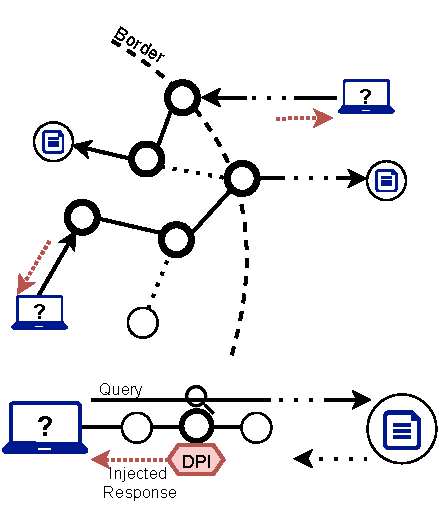
\includegraphics[width=0.8\linewidth]{figures/dns_censorship.pdf}
        \caption{DNS censorship is carried out by on-path or in-path deep packet
        inspection (DPI) appliances that monitor for block-listed keywords or
        expressions in DNS queries and inject forged responses. The original
        request and subsequent response are not typically dropped by the
        adversary, but will arrive after the forged response rendering them
        useless. DPI appliances can be deployed in local infrastructure,
        regional ISPs, or national border gateways and inject the forged response
        toward the query source in either direction.}
        \label{fig:dns_censorship}
      \end{figure}

}


%%% Local Variables:
%%% mode: latex
%%% TeX-master: "main"
%%% End:





\newcommand{\FigProbeSend}{
    \begin{figure}[t]
     \centering
     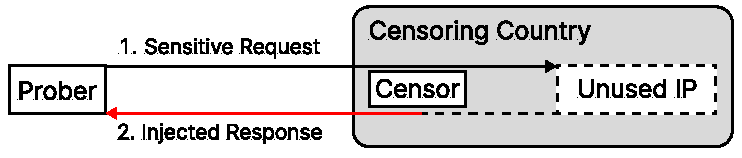
\includegraphics[width=0.95\linewidth]{figures/probe_send_02.pdf}
     \caption{\textbf{Sending Probes}\,---\,%
            For each protocol we test, we send probes to addresses from which we do not expect responses. When a passive censor monitoring traffic along the
            path to a target address is triggered by a blocklisted domain it
            injects a packet where no response would exist otherwise.}
    \label{fig:probeSend}
    \end{figure}
}


\newcommand{\FigAllocSize}{
    \begin{figure*}[t]
     \centering
     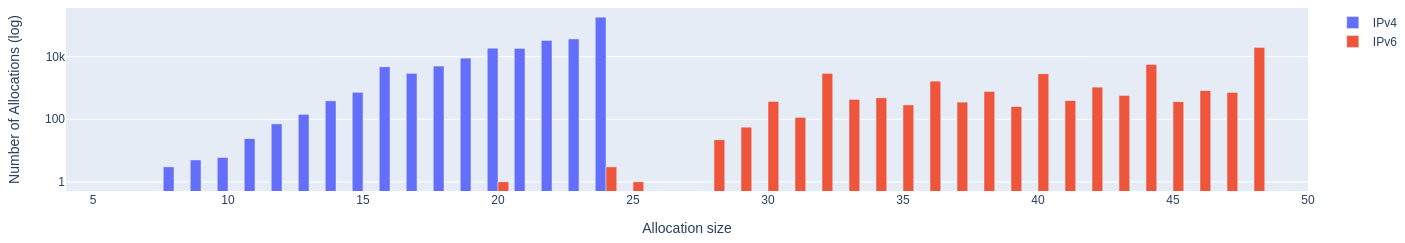
\includegraphics[width=0.95\linewidth]{figures/bgp_allocation_sizes_cropped.png}
     \caption{\textbf{Target allocation sizes}\,---\,%
            We draw our target addresses at random from BGP announced
            allocations. This graph shows the allocation sizes from which we
            select for both IPv4 and IPv6.}
    \label{fig:allocsizes}
    \end{figure*}
}


\newcommand{\PrevalenceGeneral}{\begin{table*}
\centering
\begin{tabular}{|c|l|l|c|l|c|l|} 
\hline
\multicolumn{1}{|l|}{\diagbox{\textbf{Country}}{\textbf{Protocol}}} & \textbf{DNS-A}                    & \textbf{DNS-AAAA}                 & \multicolumn{1}{l|}{\textbf{HTTP (stateful)}} & \textbf{HTTP}                    & \multicolumn{1}{l|}{\textbf{TLS (stateful)}} & \textbf{TLS}                      \\ 
\hline
\textbf{China}                                                      & \multicolumn{1}{c|}{\RIGHTcircle} & \multicolumn{1}{c|}{\RIGHTcircle} & \CIRCLE                                       & \multicolumn{1}{c|}{\LEFTcircle} & \CIRCLE                                      & \multicolumn{1}{c|}{\LEFTcircle}  \\ 
\hline
\textbf{Iran}                                                       & \multicolumn{1}{c|}{\CIRCLE}      & \multicolumn{1}{c|}{\CIRCLE}      & \CIRCLE                                       & \multicolumn{1}{c|}{}            & \RIGHTcircle                                 & \multicolumn{1}{c|}{}             \\ 
\hline
\textbf{Uzbekistan}                                                 &                                   &                                   & \CIRCLE                                       &                                  & \CIRCLE                                      &                                   \\ 
\hline
\textbf{Oman}                                                       &                                   &                                   & \CIRCLE                                       & \multicolumn{1}{c|}{\CIRCLE}     & \CIRCLE                                      &                                   \\ 
\hline
\textbf{Morocco}                                                    &                                   &                                   & \LEFTcircle                                   &                                  & \multicolumn{1}{l|}{}                        &                                   \\ 
\hline
\textbf{Bangladesh}                                                 &                                   &                                   & \CIRCLE                                       & \multicolumn{1}{c|}{\CIRCLE}     & \multicolumn{1}{l|}{}                        &                                   \\ 
\hline
\textbf{Tanzania}                                                   &                                   &                                   & \LEFTcircle                                   & \multicolumn{1}{c|}{\LEFTcircle} & \multicolumn{1}{l|}{}                        &                                   \\ 
\hline
\textbf{Kuwait}                                                     &                                   &                                   & \LEFTcircle                                   &                                  & \multicolumn{1}{l|}{}                        &                                   \\ 
\hline
\textbf{Libya}                                                      &                                   &                                   & \CIRCLE                                       & \multicolumn{1}{c|}{\CIRCLE}     & \CIRCLE                                      &                                   \\ 
\hline
\textbf{Pakistan}                                                   &                                   &                                   & \CIRCLE                                       &                                  & \CIRCLE                                      &                                   \\ 
\hline
\textbf{Lebanon}                                                    &                                   &                                   & \LEFTcircle                                   &                                  & \LEFTcircle                                  &                                   \\ 
\hline
\textbf{Turkey}                                                     &                                   &                                   & \LEFTcircle                                   &                                  & \multicolumn{1}{l|}{}                        &                                   \\
\hline
\end{tabular}
\caption{\textbf{\textbf{Global view of bidirectional censorship broken down by protocol}\,---\,}
        For each country in row \textit{i} and for each protocol in column \textit{j}, 
        \CIRCLE - represnts the presence of bidirectional censorship for IPv4 and IPv6
        \LEFTcircle - represnts the presence of bidirectional censorship for IPv4 only
        \RIGHTcircle - represnts the presence of bidirectional censorship for IPv6 only
    }
\label{fig:prevalencegeneral}
\end{table*}}


\newcommand{\TabQuack}{\begin{table}
    \centering
    \begin{tabular}{l|ccc}
       & Shared & & \\ 
       & Allocations & Quack & ProtoScan  \\
    \hline
    CN & 373                & 98\%  & 35\%       \\
    RU & 139                & 26\%  & 3\%        \\
    PK & 12                 & 92\%  & 0\%        \\
    TR & 10                 & 40\%  & 0\%        \\
    LB & 5                  & 0\%   & 0\%        \\
    IR & 1                  & 100\% & 0\%        \\
    KW & 1                  & 0\%   & 0\%
    
    \end{tabular}
    \caption{\textbf{\textbf{Quack Comparison}\,---\,} The table shows the overlap
            between our work and the Quack echo measurement project.}
    \label{tab:quack}
    \end{table}
}